%%%%%%%%%%%%%%%%%%%%%%%%%%%%%%%%%%%%%%%%%
% Masters/Doctoral Thesis 
% LaTeX Template
% Version 2.5 (27/8/17)
%
% This template was downloaded from:
% http://www.LaTeXTemplates.com
%
% Version 2.x major modifications by:
% Vel (vel@latextemplates.com)
%
% This template is based on a template by:
% Steve Gunn (http://users.ecs.soton.ac.uk/srg/softwaretools/document/templates/)
% Sunil Patel (http://www.sunilpatel.co.uk/thesis-template/)
%
% Template license:
% CC BY-NC-SA 3.0 (http://creativecommons.org/licenses/by-nc-sa/3.0/)
%
%%%%%%%%%%%%%%%%%%%%%%%%%%%%%%%%%%%%%%%%%

%----------------------------------------------------------------------------------------
%	PACKAGES AND OTHER DOCUMENT CONFIGURATIONS
%----------------------------------------------------------------------------------------

\documentclass[
11pt, % The default document font size, options: 10pt, 11pt, 12pt
%oneside, % Two side (alternating margins) for binding by default, uncomment to switch to one side
english, % ngerman for German
onehalfspacex, % Single line spacing, alternatives: onehalfspacing or doublespacing
%draft, % Uncomment to enable draft mode (no pictures, no links, overfull hboxes indicated)
%nolistspacing, % If the document is onehalfspacing or doublespacing, uncomment this to set spacing in lists to single
%liststotoc, % Uncomment to add the list of figures/tables/etc to the table of contents
%toctotoc, % Uncomment to add the main table of contents to the table of contents
%parskip, % Uncomment to add space between paragraphs
%nohyperref, % Uncomment to not load the hyperref package
headsepline, % Uncomment to get a line under the header
%chapterinoneline, % Uncomment to place the chapter title next to the number on one line
%consistentlayout, % Uncomment to change the layout of the declaration, abstract and acknowledgements pages to match the default layout
] % The class file specifying the document structure
{MastersDoctoralThesis}
\usepackage[utf8]{inputenc} % Required for inputting international characters
\usepackage[T1]{fontenc} % Output font encoding for international characters

\usepackage{mathpazo} % Use the Palatino font by default
\usepackage{amsmath,amsfonts,amsthm}
\renewcommand\bibname{References}
\usepackage{fancyhdr}
\pagestyle{fancy}
\lhead{Bhagyesh Govilkar}
\usepackage[autostyle=true]{csquotes} % Required to generate language-dependent quotes in the bibliography

%----------------------------------------------------------------------------------------
%	MARGIN SETTINGS
%----------------------------------------------------------------------------------------

\geometry{
	paper=a4paper, % Change to letterpaper for US letter
	inner=3.8cm, % Inner margin
	outer=1.9cm, % Outer margin
	bindingoffset=0cm, % Binding offset
	top=2cm, % Top margin
	bottom=2cm, % Bottom margin
	%showframe, % Uncomment to show how the type block is set on the page
}

%----------------------------------------------------------------------------------------
%	THESIS INFORMATION
%----------------------------------------------------------------------------------------

\thesistitle{UAV Smart Wing Control System - proactive control of short-period oscillations} % Your thesis title, this is used in the title and abstract, print it elsewhere with \ttitle
\supervisor{Dr. T. Glyn \textsc{Thomas}} % Your supervisor's name, this is used in the title page, print it elsewhere with \supname
\examiner{} % Your examiner's name, this is not currently used anywhere in the template, print it elsewhere with \examname
\degree{MEng Aeronautics and Astronautics} % Your degree name, this is used in the title page and abstract, print it elsewhere with \degreename
\author{Bhagyesh \textsc{Govilkar}} % Your name, this is used in the title page and abstract, print it elsewhere with \authorname
\addresses{} % Your address, this is not currently used anywhere in the template, print it elsewhere with \addressname


\keywords{} % Keywords for your thesis, this is not currently used anywhere in the template, print it elsewhere with \keywordnames
\university{\href{http://www.southampton.ac.uk}{University of Southampton}} % Your university's name and URL, this is used in the title page and , print it elsewhere with \univname
\department{\href{http://department.university.com}{Department or School Name}} % Your department's name and URL, this is used in the title page and abstract, print it elsewhere with \deptname
\group{\href{http://researchgroup.university.com}{Research Group Name}} % Your research group's name and URL, this is used in the title page, print it elsewhere with \groupname
\faculty{\href{http://faculty.university.com}{Faculty Name}} % Your faculty's name and URL, this is used in the title page and abstract, print it elsewhere with \facname

\AtBeginDocument{
\hypersetup{pdftitle=\ttitle} % Set the PDF's title to your title
\hypersetup{pdfauthor=\authorname} % Set the PDF's author to your name
\hypersetup{pdfkeywords=\keywordnames} % Set the PDF's keywords to your keywords
\hypersetup{allcolors=.}
}

\begin{document}

\frontmatter % Use roman page numbering style (i, ii, iii, iv...) for the pre-content pages

\pagestyle{plain} % Default to the plain heading style until the thesis style is called for the body content

%----------------------------------------------------------------------------------------
%	TITLE PAGE
%----------------------------------------------------------------------------------------

\begin{titlepage}
\begin{center}

\vspace*{.06\textheight}
{\scshape\LARGE \univname\par}\vspace{1.5cm} % University name

\HRule \\[0.4cm] % Horizontal line
{\huge \bfseries \ttitle\par}\vspace{0.4cm} % Thesis title
\HRule \\[1.5cm] % Horizontal line
 
\begin{minipage}[t]{0.4\textwidth}
\begin{flushleft} \large
\emph{Author:}\\
{\authorname} % Author name - remove the \href bracket to remove the link
\end{flushleft}
\end{minipage}
\begin{minipage}[t]{0.4\textwidth}
\begin{flushright} \large
\emph{Supervisor:} \\
{\supname} % Supervisor name - remove the \href bracket to remove the link  
\end{flushright}
\end{minipage}\\[3cm]
\begin{center}

\includegraphics[scale=0.3]{crest.jpg}		% University/department logo - uncomment to place it
\end{center}

\large \textit{This report is submitted in partial fulfillment of the
requirements for the MEng Aeronautics and Astronautics, Faculty of Engineering and the
Environment, University of Southampton}\\[0.3cm] % University requirement text

 
\vfill

{\large \today}\\[4cm] % Date

 
\vfill
\end{center}
\end{titlepage}

%----------------------------------------------------------------------------------------
%	DECLARATION PAGE
%----------------------------------------------------------------------------------------

\section*{Declaration}
\thispagestyle{fancy}
 I, Bhagyesh Govilkar declare that this thesis and the work presented in it are my own and has
been generated by me as the result of my own original research.
I confirm that:
\begin{enumerate}
\item  This work was done wholly or mainly while in candidature for a degree at this
University;
\item  Where any part of this thesis has previously been submitted for any other
qualification at this University or any other institution, this has been clearly stated;
\item  Where I have consulted the published work of others, this is always clearly
attributed;
\item  Where I have quoted from the work of others, the source is always given. With
the exception of such quotations, this thesis is entirely my own work;
\item  I have acknowledged all main sources of help;
\item  Where the thesis is based on work done by myself jointly with others, I have
made clear exactly what was done by others and what I have contributed myself;
\item  None of this work has been published before submission.
\end{enumerate}
 

\cleardoublepage


\section*{Introduction}
\thispagestyle{fancy}
Unmanned Aerial Vehicles are becoming increasingly mainstream. With faster and more efficient ways of manufacturing such as 3D printing gaining momentum, this will only serve to bolster the emerging market. The University of Southampton's SULSA project (Southampton University Laser Sintered Aircraft) produced an UAV that was made entirely from 3D printed parts. 

There are several contemporary and potential applications of UAVs: they are widely used in agriculture to give farmers a detailed picture of the health of their farm, the amount of resources such as pesticides required and they can help cut down on labour costs; they are already being used in the defence sector mostly to carry out surveillance and reconnaissance activities, a handful are being used for offensive operations such as the MQ-9 Reaper. 

With this increasing usage of UAVs, there is a strong need for a control system that can give the user a stable, reliable and robust aircraft. The aim is to reduce the frequency of UAVs crashing, increase the life-span and reduce the maintenance costs. 

In this project, I will be looking specifically at a phenomenon known as a "short-period oscillation". This is one of the two longitudinal dynamic modes that occur on every aircraft, the other being a "phugoid oscillation". Short-period oscillations are characterised by the rapid decay and high frequency. A typical SPO can settle within a second and occurs at 1-2Hz. A pilot can induce a SPO by a sharp pitch input. They can also naturally occur due to a gust (impulsive increase/decrease in airspeed and/or angle of attack). 

A UAV control system that does not have a SPO model is vulnerable to growing instability. It can act to reinforce the oscillation instead of canceling them. Thus it is important to systematically analyse and design a model that can handle a SPO.  
\newpage
%----------------------------------------------------------------------------------------
%	ACKNOWLEDGEMENTS
%----------------------------------------------------------------------------------------
\begingroup
\let\clearpage\relax
\let\cleardoublepage\relax
\begin{acknowledgements}
\thispagestyle{fancy}
 % Add the acknowledgements to the table of contents
I would like to acknowledge my supervisor, Dr T. Glyn Thomas who provided me with guidance every step of the way and supported my ideas that enabled me to complete this project.\ldots

\end{acknowledgements}
\endgroup
\newpage
%----------------------------------------------------------------------------------------
%	ABBREVIATIONS
%----------------------------------------------------------------------------------------
\begingroup
\let\clearpage\relax
\let\cleardoublepage\relax
\begin{abbreviations}{ll} % Include a list of abbreviations (a table of two columns)
\thispagestyle{fancy}
\textbf{LAH} & \textbf{L}ist \textbf{A}bbreviations \textbf{H}ere\\
\textbf{WSF} & \textbf{W}hat (it) \textbf{S}tands \textbf{F}or\\

\end{abbreviations}
\endgroup
\newpage
%----------------------------------------------------------------------------------------
%	PHYSICAL CONSTANTS/OTHER DEFINITIONS
%----------------------------------------------------------------------------------------
\begingroup
\let\clearpage\relax
\let\cleardoublepage\relax
\begin{constants}{lr@{${}={}$}l} % The list of physical constants is a three column table
\thispagestyle{fancy}
% The \SI{}{} command is provided by the siunitx package, see its documentation for instructions on how to use it

Speed of Light & $c_{0}$ & \SI{2.99792458e8}{\meter\per\second} (exact)\\
%Constant Name & $Symbol$ & $Constant Value$ with units\\

\end{constants}
\endgroup
\newpage
%----------------------------------------------------------------------------------------
%	SYMBOLS
%----------------------------------------------------------------------------------------
\begingroup
\let\clearpage\relax
\let\cleardoublepage\relax
\begin{symbols}{lll} % Include a list of Symbols (a three column table)
\thispagestyle{fancy}
$a$ & distance & \si{\meter} \\
$P$ & power & \si{\watt} (\si{\joule\per\second}) \\
%Symbol & Name & Unit \\

\addlinespace % Gap to separate the Roman symbols from the Greek

$\omega$ & angular frequency & \si{\radian} \\

\end{symbols}
\endgroup
\newpage
\tableofcontents

%----------------------------------------------------------------------------------------
%	THESIS CONTENT - CHAPTERS
%----------------------------------------------------------------------------------------

\mainmatter % Begin numeric (1,2,3...) page numbering

\pagestyle{plain} % Return the page headers back to the "thesis" style

% Include the chapters of the thesis as separate files from the Chapters folder
% Uncomment the lines as you write the chapters

\chapter{Current state-of-the-art}
The knowledge we currently have and the applications of this knowledge need to be established first to identify the areas in which we lack an understanding and where improvements and optimisations can be made. In this chapter, I intend to do exactly that. By the end of this chapter, it will be clear that there has been little development in this area. 

\section{Flight dynamics}

We need to understand flight dynamics to determine the modes of longitudinal oscillations.

I will use the longitudinal equations of motion as a starting point :
$$\begin{bmatrix}\Delta\dot{u}\\\dot{w}\\\dot{q}\\\Delta\dot{\theta}\end{bmatrix} =$$
$$ \begin{bmatrix}\frac{\mathring{X}_{u}}{m}&\frac{\mathring{X}_{w}}{m}&0&-gcos\theta_{0}\\\frac{\mathring{Z}_{u}}{m-\mathring{Z}_{\dot{w}}}&\frac{\mathring{Z}_{w}}{m-\mathring{Z}_{\dot{w}}}&\frac{\mathring{Z}_{q}+mU_{\infty}}{m-\mathring{Z}_{\dot{w}}}&\frac{-mgsin\theta_{0}}{m-\mathring{Z}_{\dot{w}}}\\\frac{1}{I_{y}}\left[\mathring{M}_{u}+\frac{\mathring{M}_{\dot{w}}\mathring{Z_{u}}}{m-\mathring{Z}_{\dot{w}}}\right]&\frac{1}{I_{y}}\left[\mathring{M}_{w}+\frac{\mathring{M}_{\dot{w}}\mathring{Z_{u}}}{m-\mathring{Z}_{\dot{w}}}\right]&\frac{1}{I_{y}}\left[\mathring{M}_{q}+\frac{\mathring{M}_{\dot{w}}(\mathring{Z_{q}}+mU_{\infty})}{m-\mathring{Z}_{\dot{w}}}\right]&-\frac{M_{\dot{w}}mg\sin(\theta_{0})}{I_{y}(m-Z_{\dot{w}})}\\0&0&1&0\end{bmatrix}\begin{bmatrix}\Delta u\\w\\q\\\Delta\theta\end{bmatrix}+$$
$$\begin{bmatrix}\frac{\Delta \mathring{X_{c}}}{m}\\\frac{\Delta \mathring{Z_{c}}}{m-\mathring{Z}{\dot{w}}}\\\frac{\Delta \mathring{M}_{c}}{I_{y}} + \frac{\mathring{M}_{\dot{w}}}{I_{y}}\frac{\Delta \mathring{Z_{c}}}{m-\mathring{Z}{\dot{w}}}\\0\end{bmatrix}$$ 

The derivation of these equations are fairly straightforward but quite lengthy and can be found in virtually any flight mechanics/dynamics textbook \cite{etkin}.

These equations can be rewritten in the form:
$$\dot{\textbf{x}} = \textbf{Ax+B}$$
Where $x$ is the state vector, $\textbf{A}$ is the system matrix (constant) and B is a vector of control forces and moments which can be considered 0.
$$\dot{\textbf{x}}=\textbf{Ax}$$
This is a first order ODE which means that the solutions are in the form of $$\textbf{x}=\textbf{x}_{0}e^{\lambda t}$$
$$\lambda\textbf{x}_{0}=\textbf{Ax}_{0}$$
$$(\textbf{A}-\lambda\textbf{I})\textbf{x}_{0}=0$$
Non-trivial solutions occur when $det(\textbf{A}-\lambda\textbf{I})=0$. Solving this equation for any given aircraft will give a quartic equation (4th order polynomial) which when solved will give two pairs of complex conjugates. One of the pairs corresponds to the phugoid mode while the other one corresponds to the SPO. 

For example, we can consider the Navion aircraft \cite{navion}:

$$\textbf{A} = \begin{bmatrix}
-0.09148&0.04242&0&-32.17\\
10.51&-3.066&152&0\\
0.2054&-0.05581&-2.114&0\\
0&0&1&0
\end{bmatrix}$$
Computing the eigenvalue of this matrix:
\begin{figure}[h]
\centering
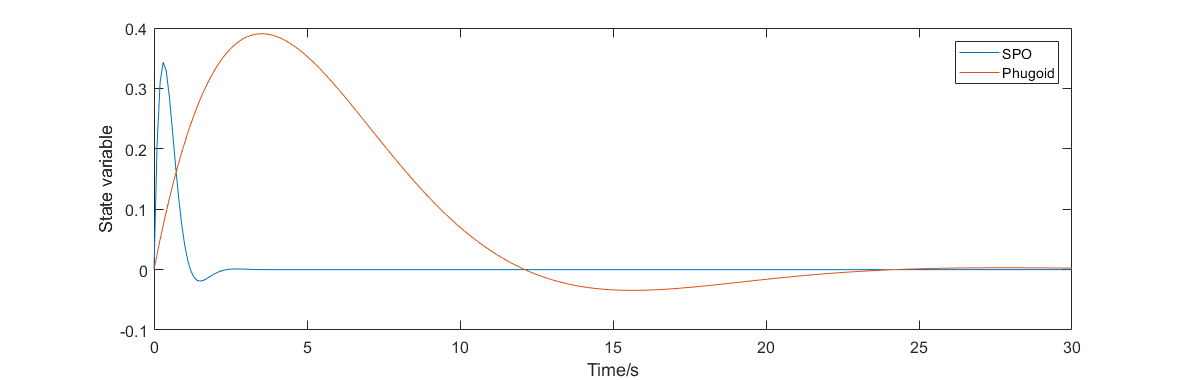
\includegraphics[scale=0.6]{DI.png}
\caption{MATLAB output}
\centering
\end{figure}
The matrix produces two pairs of complex conjugate eigenvalues. The first pair $\lambda_{1,2}= -2.4352 \pm 2.6461i$ is the SPO mode. The decay rate (the real part) is much greater than the other pair $\lambda_{3,4} = -0.2006 \pm 0.2593i$ and so is the frequency (coefficient of i). 
\section{Mitigation of longitudinal dynamic modes}

\subsection{SPO regulations and qualification}
The United States of America's Federal Aviation Authority regulates SPOs in FAR Part 23.181 \cite{far} as follows:
Any short period oscillation not including combined lateral-directional oscillations occurring between the stalling speed and the maximum allowable speed appropriate to the configuration of the airplane must be heavily damped with the primary controls -

(1) Free; and

(2) In a fixed position.
\newline
United Kingdom's Civil Aviation Authority regulates SPOs in a very similar manner and can be found in CAP482 S181. 

The quality of handling is largely determined by pilot opinion. This is visualised by pilot opinion charts such as the one shown below. 
\begin{figure}[h]
\centering
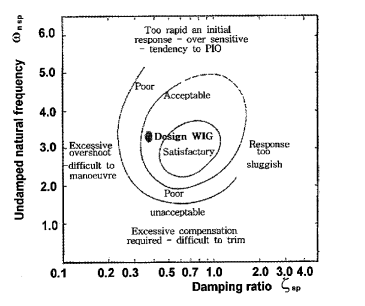
\includegraphics[scale=1]{contour.png}
\caption{Short-period pilot opinion contours \cite{chung}}
\centering
\end{figure}

From SPO approximation \cite{short} we can determine the natural frequency and damping ratio:
$$\omega_{n}=\sqrt{\mathring{Z}_{w}\mathring{M}_{q}+\mathring{M}_{w}\mathring{Z}_{q}}$$
$$\zeta = \frac{\mathring{M}_{q}+\mathring{Z}_{w}}{\omega_{n}}$$
Therefore, simply by adjusting the aerodynamic derivatives, it is possible to conform to the regulations. The regulations do not make the existence of a control system with a SPO dedicated model mandatory. This is most likely the reason why no such system exists. Thus, to fill this gap I will be developing a system that will focus on minimising the impact of SPOs.  
\thispagestyle{fancy}
\subsection{Phugoid suppression}
It is worth looking at how we deal with Phugoid oscillations first since suppressing phugoid oscillations has been well documented. This is achieved through the use of a Pitch Attitude Controller and has been described by Etkin in \textit{Dynamics of Flight Stability and and Control} \cite{etkin}. More recently, in the paper \textit{Pitch Attitude Controller Design and Simulation for a Small Unmanned Aerial Vehicle} \cite{huang} a pitch-rate feedback control system was explored. In both cases, the control system did well to suppress Phugoid oscillations and managed to weaken SPOs but relied on gyroscopes or other attitude sensors. This meant that the control system took action AFTER the flight dynamics caused a deviation in the pitch rate/angle from the nominal. This model is currently the state-of-the-art, but includes an intrinsic lag between the onset of the oscillations and the corrective action of the controller.  

There has been little development in designing a control system that detects the disturbance at the source and takes action BEFORE the flight dynamics can cause an appreciable change in attitude. In this project, I will aim to achieve a control system that does not wait for a large change in attitude to occur before acting. This will hopefully reduce the amplitude of the oscillation and the associated risks. 
\chapter{Method}
In this chapter, major design decisions and developing the tools required for this project will be discussed. There are for major decisions that need to be made: Pressure sensors, actuators, micro-controller, and the programming language. 
\section{Pressure sensors}
There are a variety of sensors to choose from. There are absolute pressure sensors that simply measure the gauge or absolute pressure. Then there are pressure sensors that measure differential pressure. These have two ports and the sensor will measure the difference in pressure between them. 

To calculate the lift on the wing, we will need to know the pressure distribution along the top and the bottom of the wing. A single differential pressure sensor can tell the difference in pressure at a certain chord position on the wing. For the same information, two absolute pressure sensors will be required. Furthermore, the airspeed in the wind tunnel will need to be measured. Using a differential sensor, one port can be subjected to the total/stagnation pressure from a pitot probe, and the second port will be subjected to the static pressure. The sensor will instantly give the difference between the two pressures which is the dynamic pressure. The airspeed can then be easily calculated using Bernoulli's principle: $$V=\sqrt{\frac{2(p_{0}-p)}{\rho}}$$

Thus, for convenience a differential type sensor will be used. TE connectivity makes a sensor called MS4524DO in both differential and absolute flavours. There is also the option to choose between the I2C and SPI data transmission buses. 

There are merits to using both buses. The I2C bus is very common and many devices use it to communicate with a 'master'. The bus typically runs at 100kbps but can reach 400kbps on fast mode. It uses a data line (SDA) and a clock line (SCL) and is therefore sometimes called 'two wire interface' (TWI). 

SPI on the other hand runs much faster at around 10Mbps. The interface requires a clock line (SCLK), a MISO line (Master in Slave out), sometimes a MOSI line (Master out Slave in) and a slave select pin. 

The slave select pin allows communication with a specific device on the line. In this case, we will have four pressure sensors but we will need to talk to one sensor before moving on to the next. 

I2C relies on the device address. Each I2C device is given a specific address which needs to be provided before data transmission can happen. All available I2C MS4525DO sensors have the address 0x28 which creates a conflict. The I2C bus will not know which sensor to communicate with because they're all at the same address. A 'switching' mechanism will be needed to make this option viable. 

The most suitable bus for this application is obviously SPI. However, there is a severe lack of availability of these sensors at a reasonable price. A compromise in speed had to be made by choosing the I2C sensor which are widely available. However, for our purpose the speed exceeds Nyquist criterion (test described in chapter) so the lower bus speed will not be an issue. 
\thispagestyle{fancy}
\newpage
%----------------------------------------------------------------------------------------
%	BIBLIOGRAPHY
%----------------------------------------------------------------------------------------
\renewcommand{\bibname}{References}
\begin{thebibliography}{9}
\addcontentsline{toc}{chapter}{References}
\bibitem{navion} 
Catterall, R. (2003). State-Space Modeling of the Rigid-Body Dynamics of a Navion Airplane From Flight Data, Using Frequency-Domain Identification Techniques. [online] Trace.tennessee.edu. Available at: \url{http://trace.tennessee.edu/cgi/viewcontent.cgi?article=3269&context=utk_gradthes} [Accessed 2 Feb. 2018].
 
\bibitem{etkin}

B. Etkin and L. Reid, Dynamics of flight. Chichester: Wiley, 1996, pp. 15, 174,175.
 
\bibitem{chung} 
H. Chun and C. Chang, "Longitudinal stability and dynamic motions of a small passenger WIG craft", Ocean Engineering, vol. 29, no. 10, p. 1161, 2002.

\bibitem{huang}
C. Huang, Q. Shao, P. Jin, Z. Zhu and B. Zhang, "Pitch Attitude Controller Design and Simulation for a Small Unmanned Aerial Vehicle," 2009 International Conference on Intelligent Human-Machine Systems and Cybernetics, Hangzhou, Zhejiang, 2009, 
URL: \url{http://ieeexplore.ieee.org/stamp/stamp.jsp?tp=&arnumber=5336043&isnumber=5335881}
\bibitem{far}
"14 CFR 23.181 - Dynamic stability.", LII / Legal Information Institute, 2011. [Online]. Available: https://www.law.cornell.edu/cfr/text/14/23.181. [Accessed: 03- Feb- 2018].
\bibitem{short}
B. Aliyu, C. Osheku, P. Okeke, F. Opara and B. Okere, "Oscillation Analysis for Longitudinal Dynamics of a Fixed-Wing UAV Using PID Control Design", Advances in Research, vol. 5, no. 3, p. 6, 2015.
\end{thebibliography}


%----------------------------------------------------------------------------------------
%----------------------------------------------------------------------------------------
%	THESIS CONTENT - APPENDICES
%----------------------------------------------------------------------------------------

\appendix % Cue to tell LaTeX that the following "chapters" are Appendices

% Include the appendices of the thesis as separate files from the Appendices folder
% Uncomment the lines as you write the Appendices

% Appendix A
\chapter{Manufacturing and assembly}

The main wing was split into four parts: the two ends of the wings, the middle section (as shown in figure 4.1) and the flap. Different manufacturing processes had to be utilised to obtain these parts quickly and of sufficient quality. 

\thispagestyle{fancy}
The middle section is geometrically complex due to the presence of the pressure tappings. It is not very practical to hand craft the part and not feasible through 2D processes such as laser cutting or foam cutting due to the 3D geometric features. 3D printing is the only process that is suitable and available for this component. Unfortunately, the span of the wing is too great (30cm) for the 3D printer so to ends of the wing need to be extended. The 3D printed part was made 20cm wide. 

To extend the wing by 5cm each side, the profile of the middle section was saved as a .dxf file. This profile was laser cut out of a 5mm thick plywood 20 times and glued together side-to-side. 

The flap was made similarly. The profile was laser cut 60 times and glued together. 

The main wing has been supported and mounted through two 6mm carbon fibre rods that go through the wing and attach to some fixtures on the walls of the tunnel. These fixtures were designed specifically for this project. 
\begin{figure}[H]
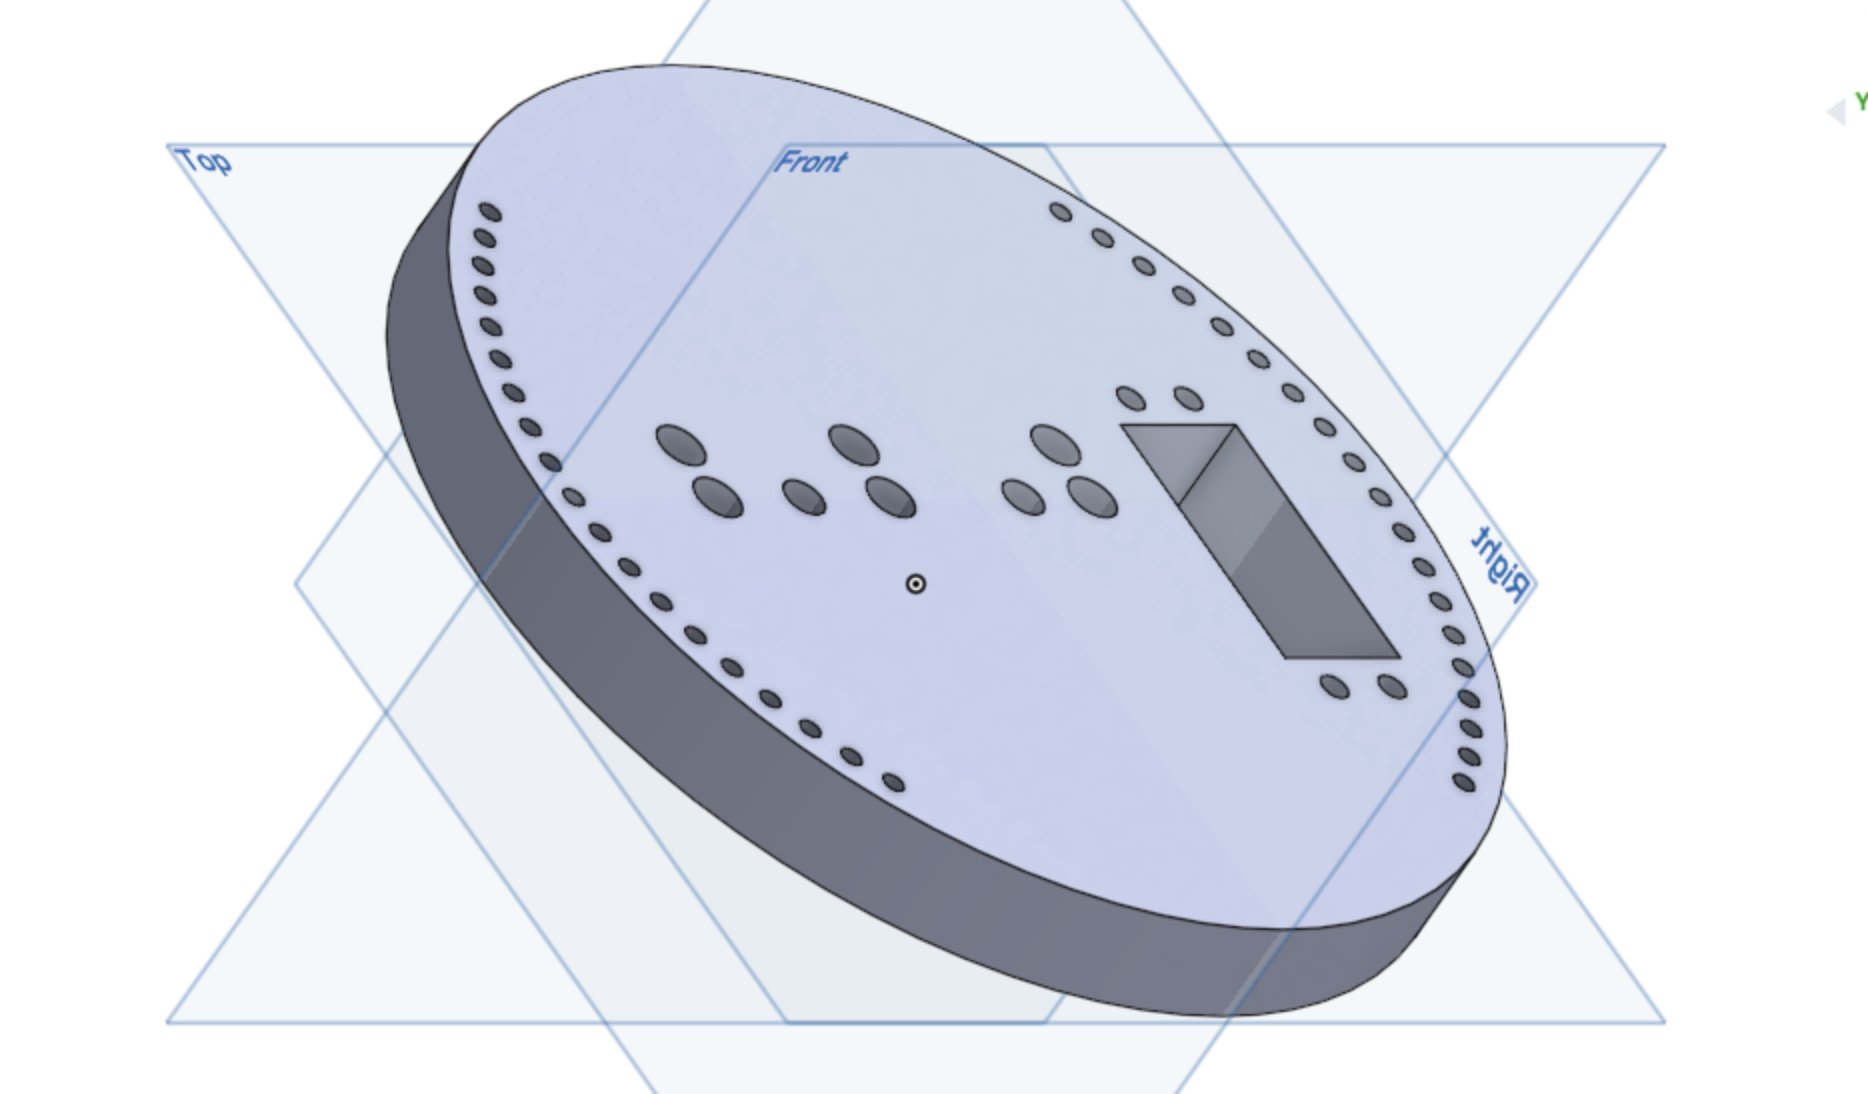
\includegraphics[scale=0.45]{fix.png}
\caption{Fixture on the right hand side of the wind tunnel}
\end{figure}
Looking upstream, the fixture disc on the right hand side (Figure 4.3) has holes for the carbon fibre rods, a cut out for the flap servo to be mounted in, six holes for the PVC tubes connecting the pressure tappings to the sensors and several holes near the edges to allow changing the angle of attack of the wing to a desired setting. The angular separation between these holes is 5$^{\circ}$. 
\thispagestyle{fancy}
\begin{figure}[h]
\centering
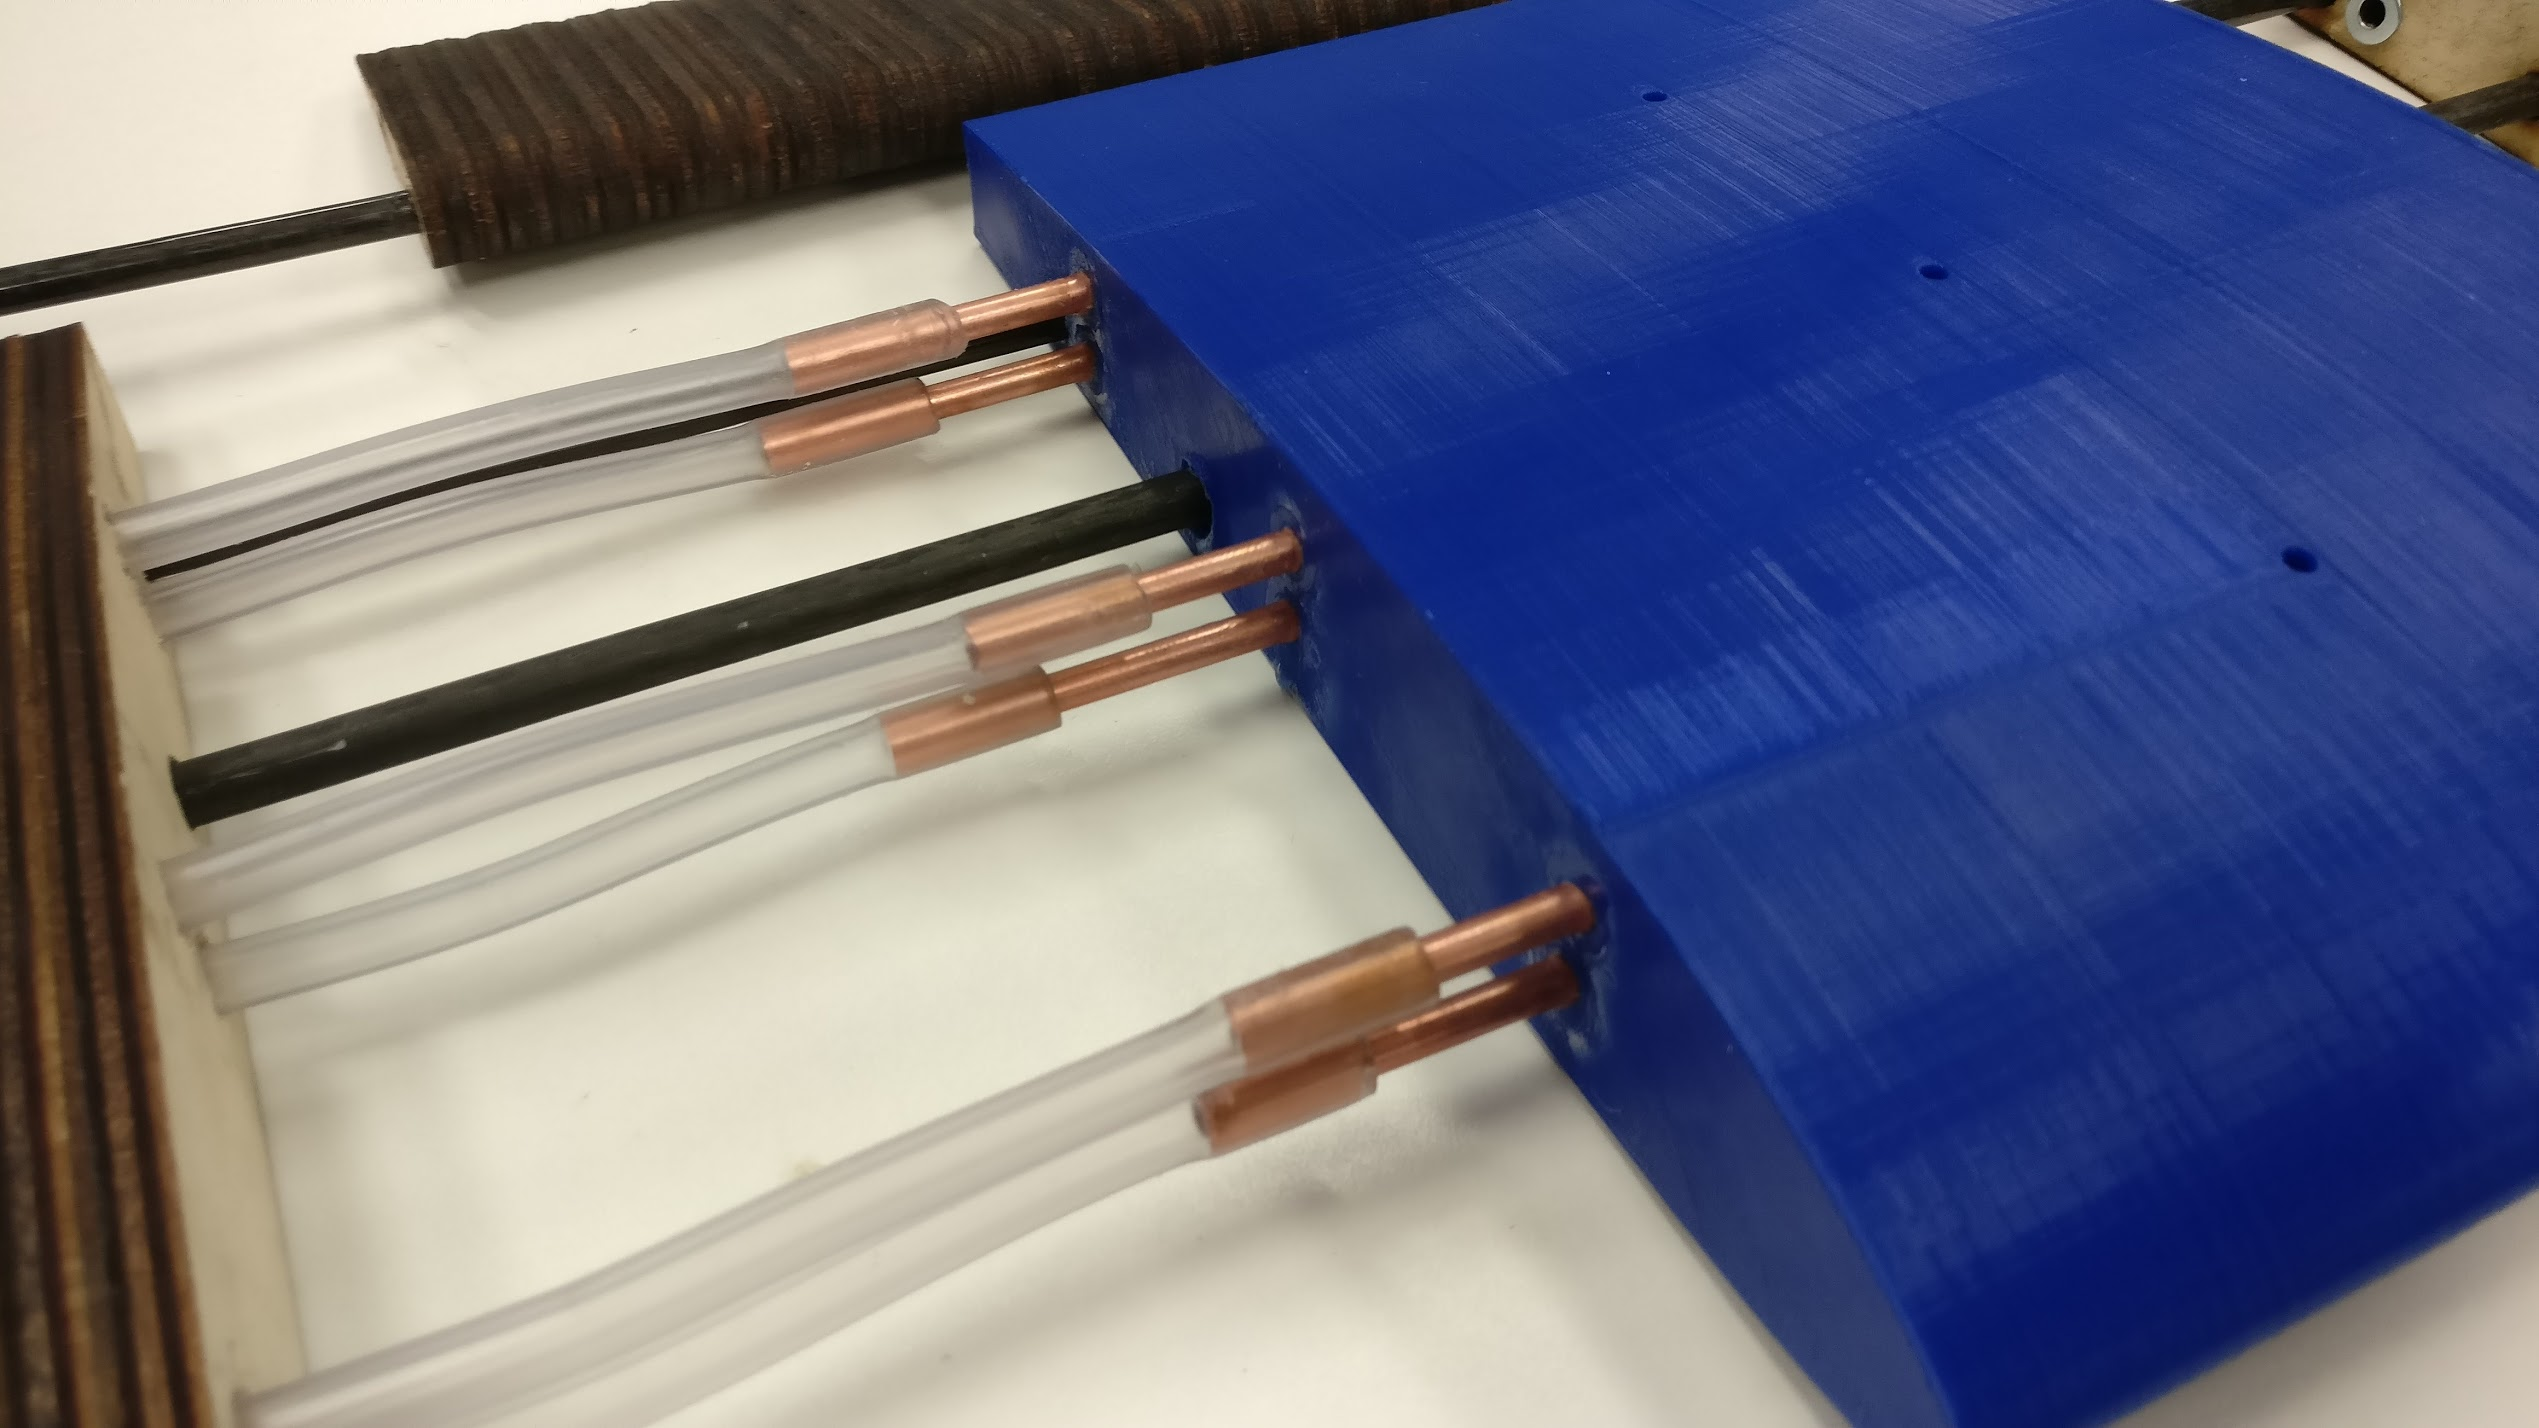
\includegraphics[scale=0.1]{pipe.jpg}
\caption{Picture of the PVC tubing and the midsection of the wing}
\centering
\end{figure}
The pressure tappings end at the right side of the middle section of the wing. Sections of a 4mm (outer diameter) copper pipe were placed in these holes and glued in place. \thispagestyle{fancy} These created "ports" which allowed easy and secure connection of the pressure tappings to the pressure sensors. Six equal sections of 3mm PVC tube(inner diameter) were cut to facilitate this connection. One end of each tube was secured to the pressure sensor ports, the other end had to be heated and expanded to fit onto the larger copper ports on the wing. This provided an excellent tight seal which is beneficial because less pressure will be lost. 
\thispagestyle{fancy}

\thispagestyle{fancy}
\newpage
\begin{figure}[H]
\centering
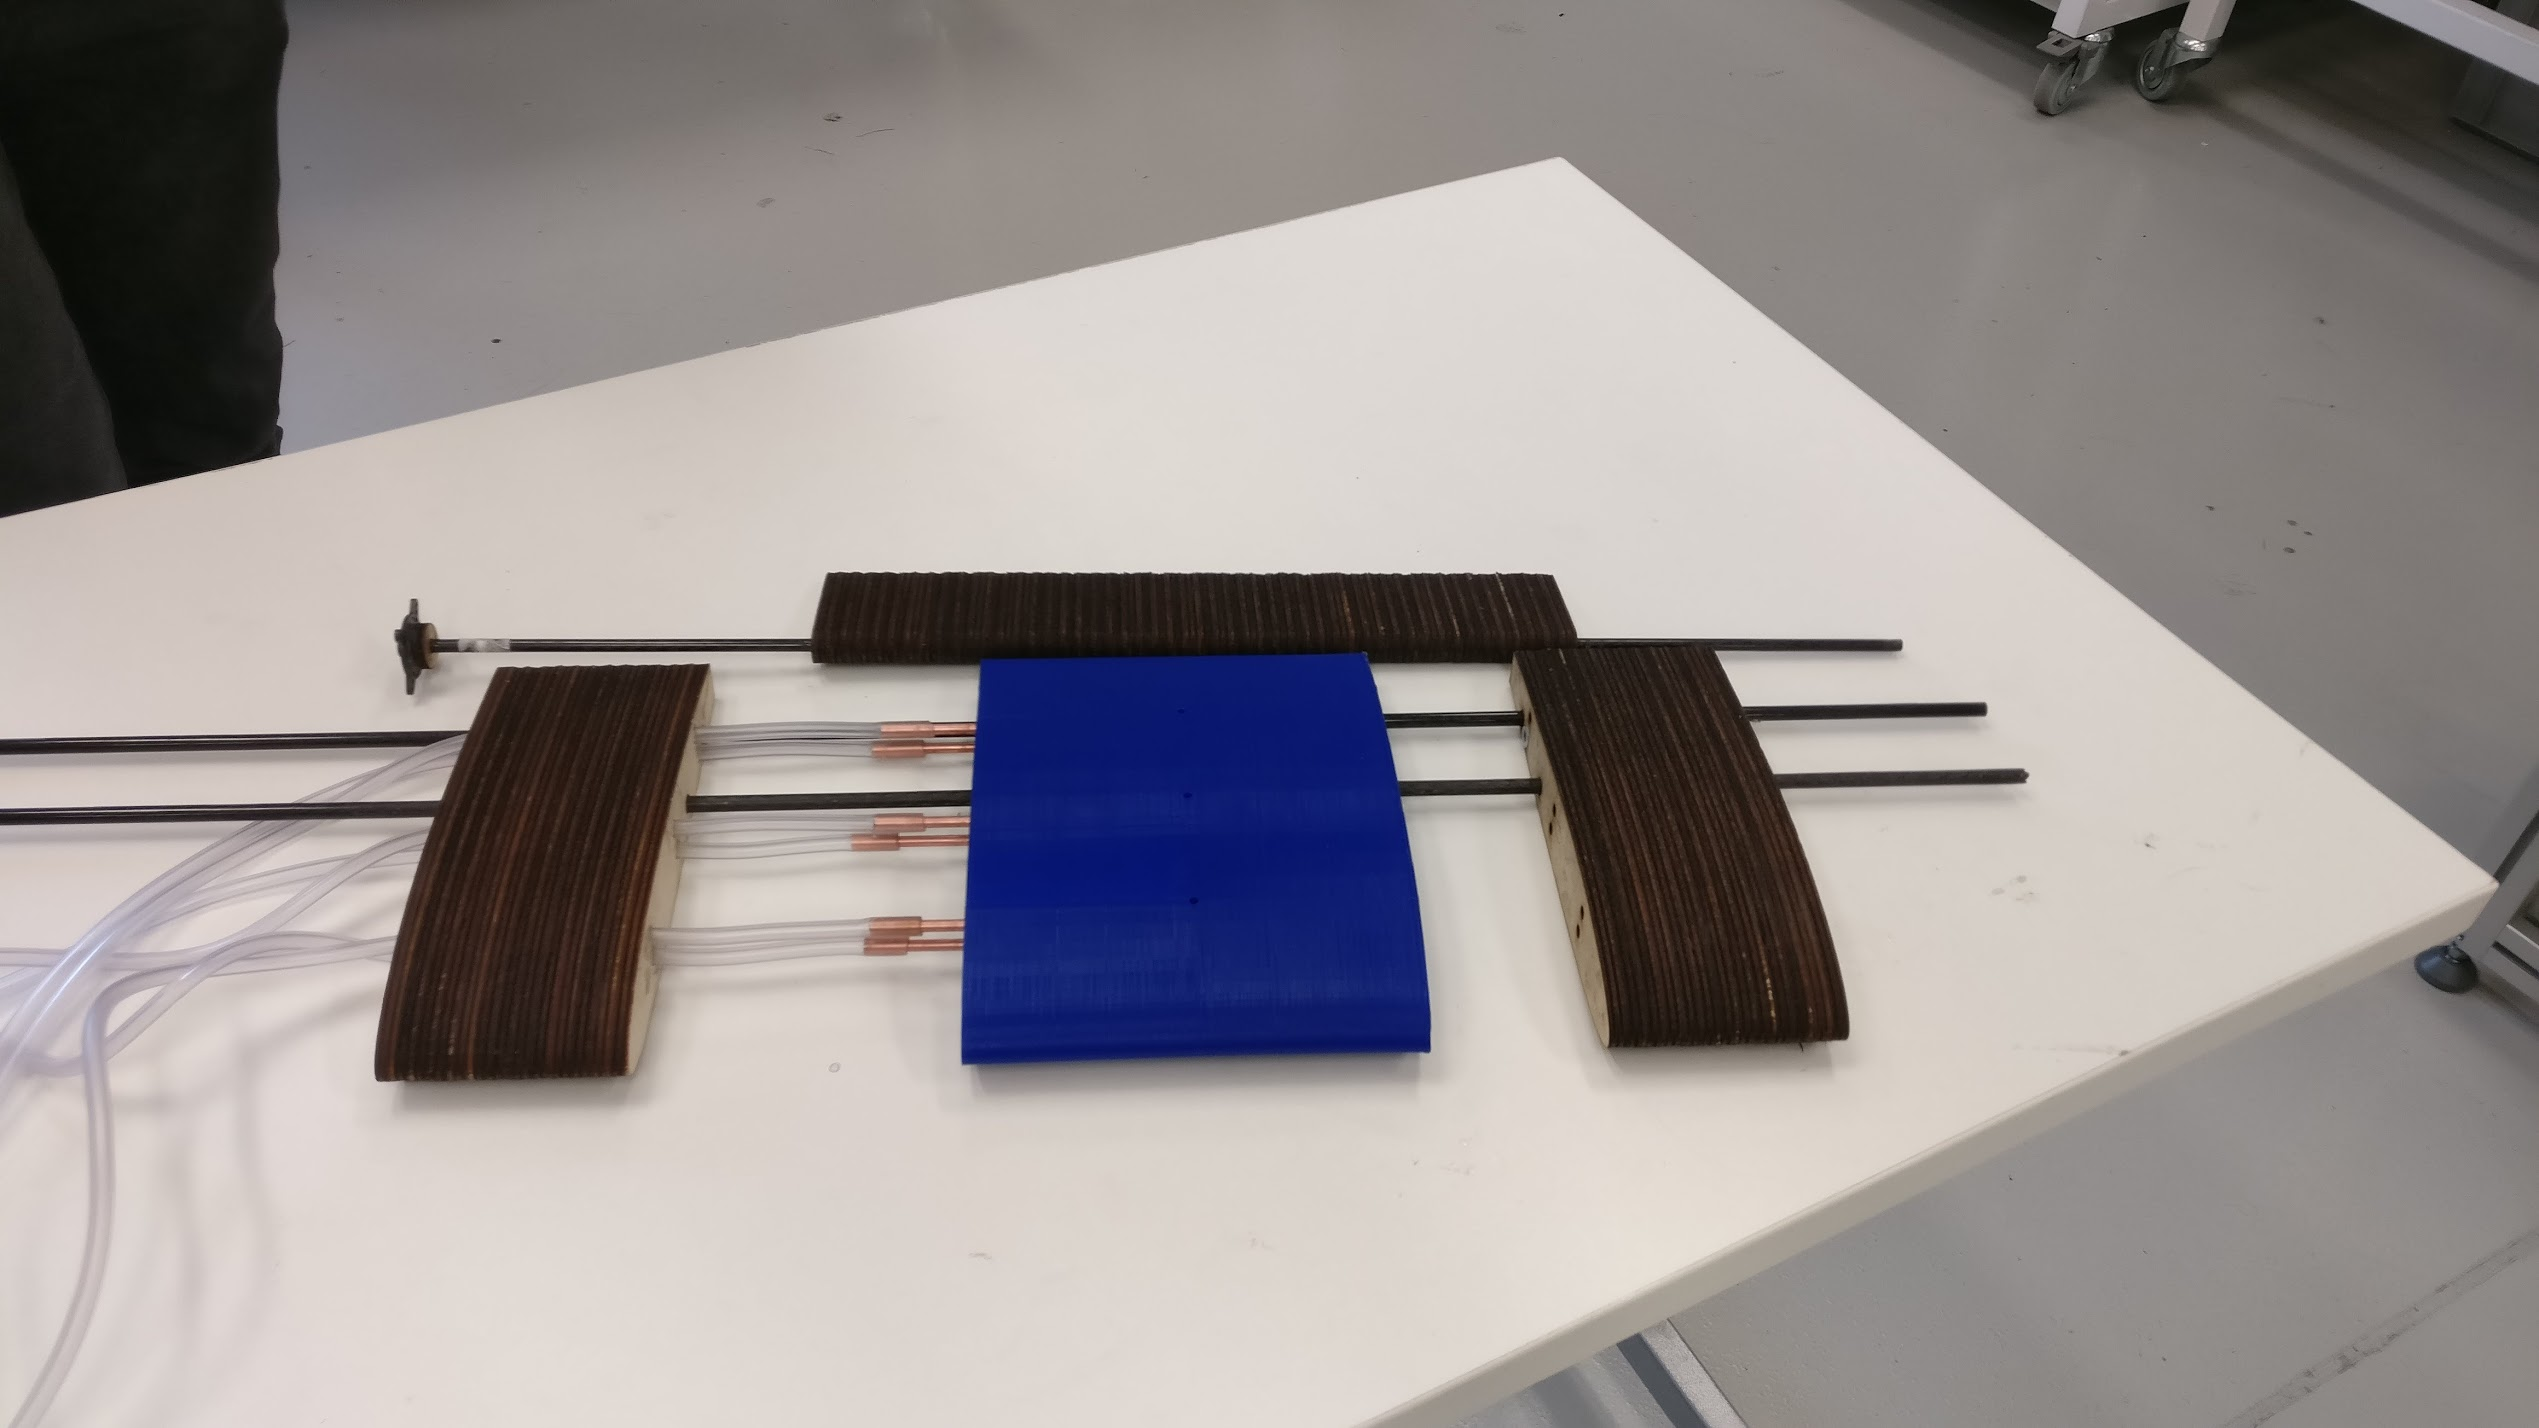
\includegraphics[scale=0.12]{integ.jpg}
\caption{Picture showing how the different parts of the wing were integrated}
\centering
\end{figure}
\begin{figure}[H]
\centering
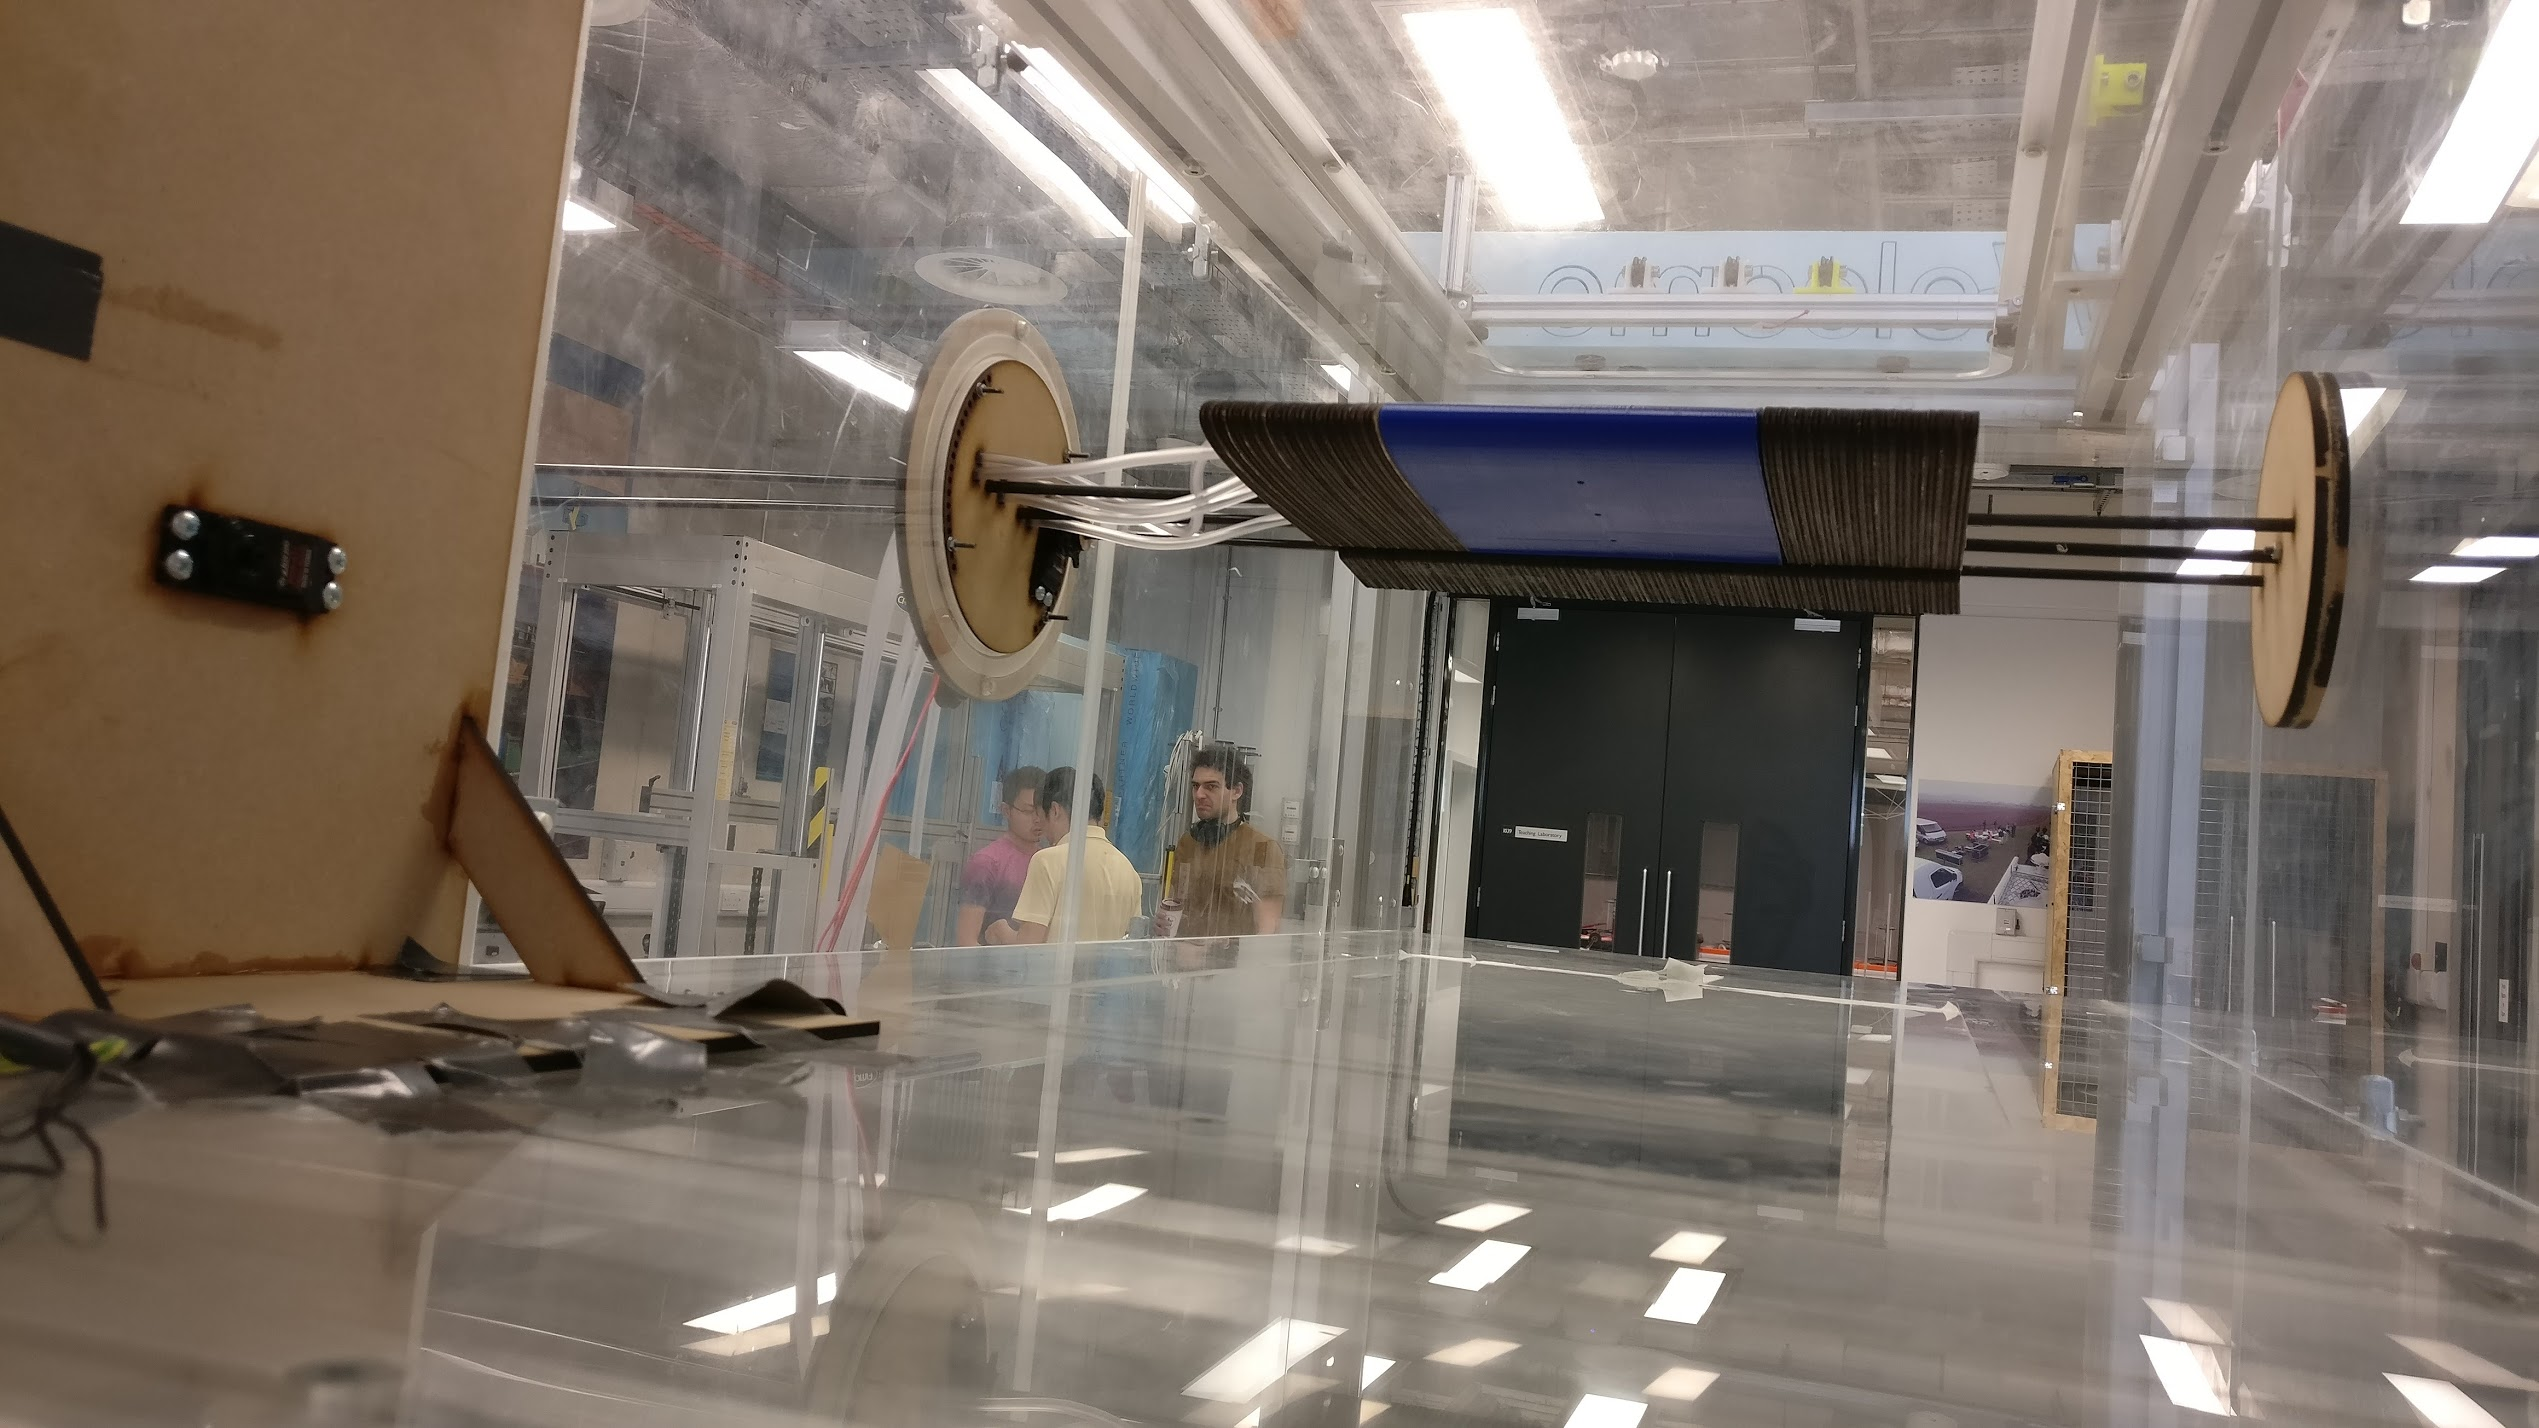
\includegraphics[scale=0.15]{wind.jpg}
\caption{Picture showing the main wing assembly in the wind tunnel}
\centering
\end{figure}

\chapter{Risk Assessment} % Main appendix title
\thispagestyle{fancy}
\begin{figure}[H]
\centering
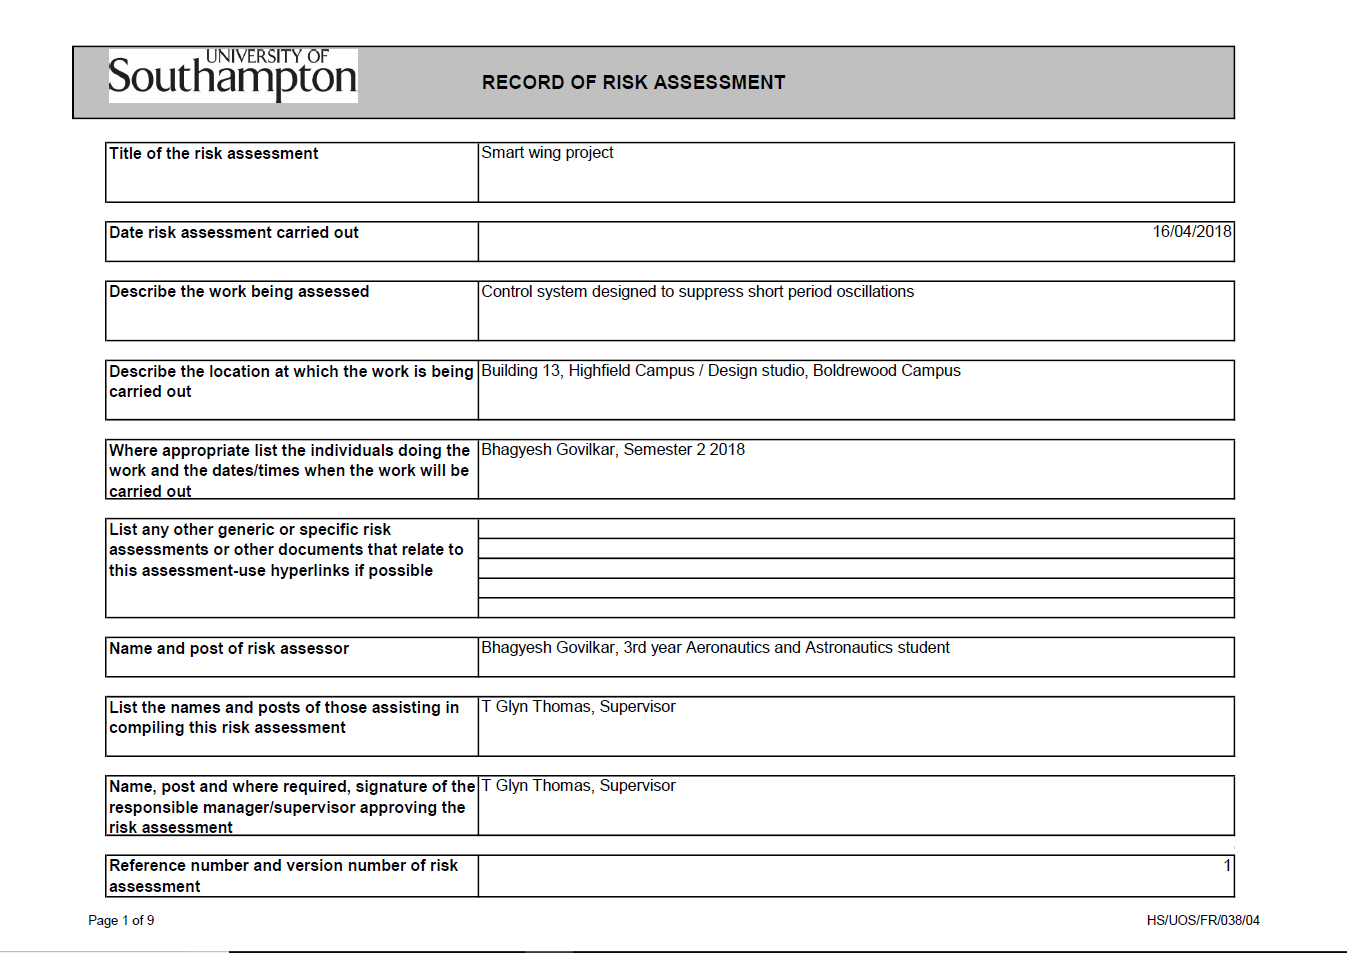
\includegraphics[scale=0.5]{ra1.png}
\caption{Section A}
\centering
\end{figure}
\newpage
\begin{sidewaysfigure}
\centering
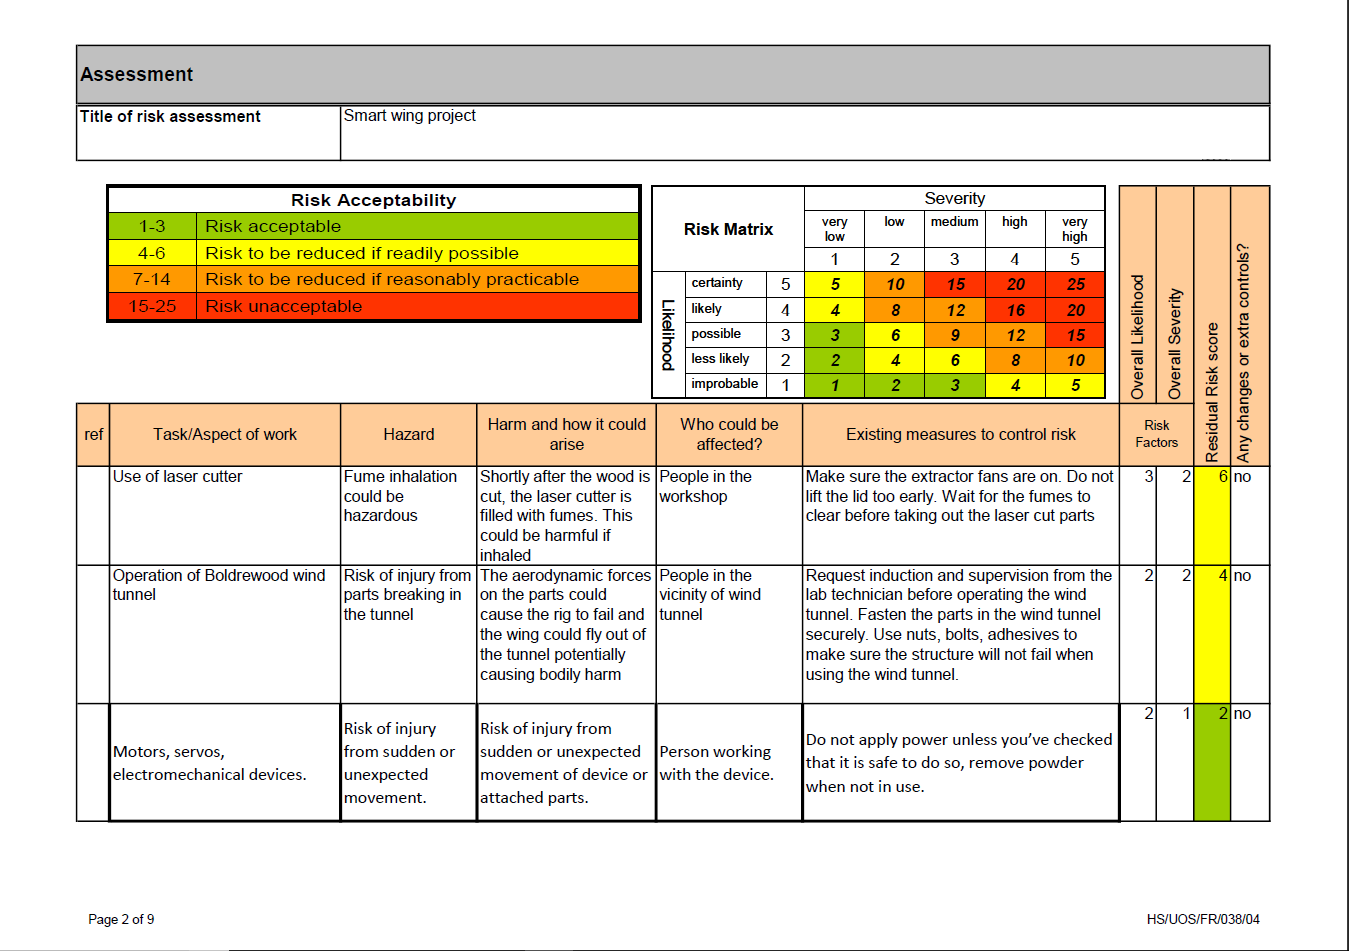
\includegraphics[scale=0.6]{ra2.png}
\caption{Section B}
\centering
\end{sidewaysfigure}
\newpage
\begin{sidewaysfigure}
\centering
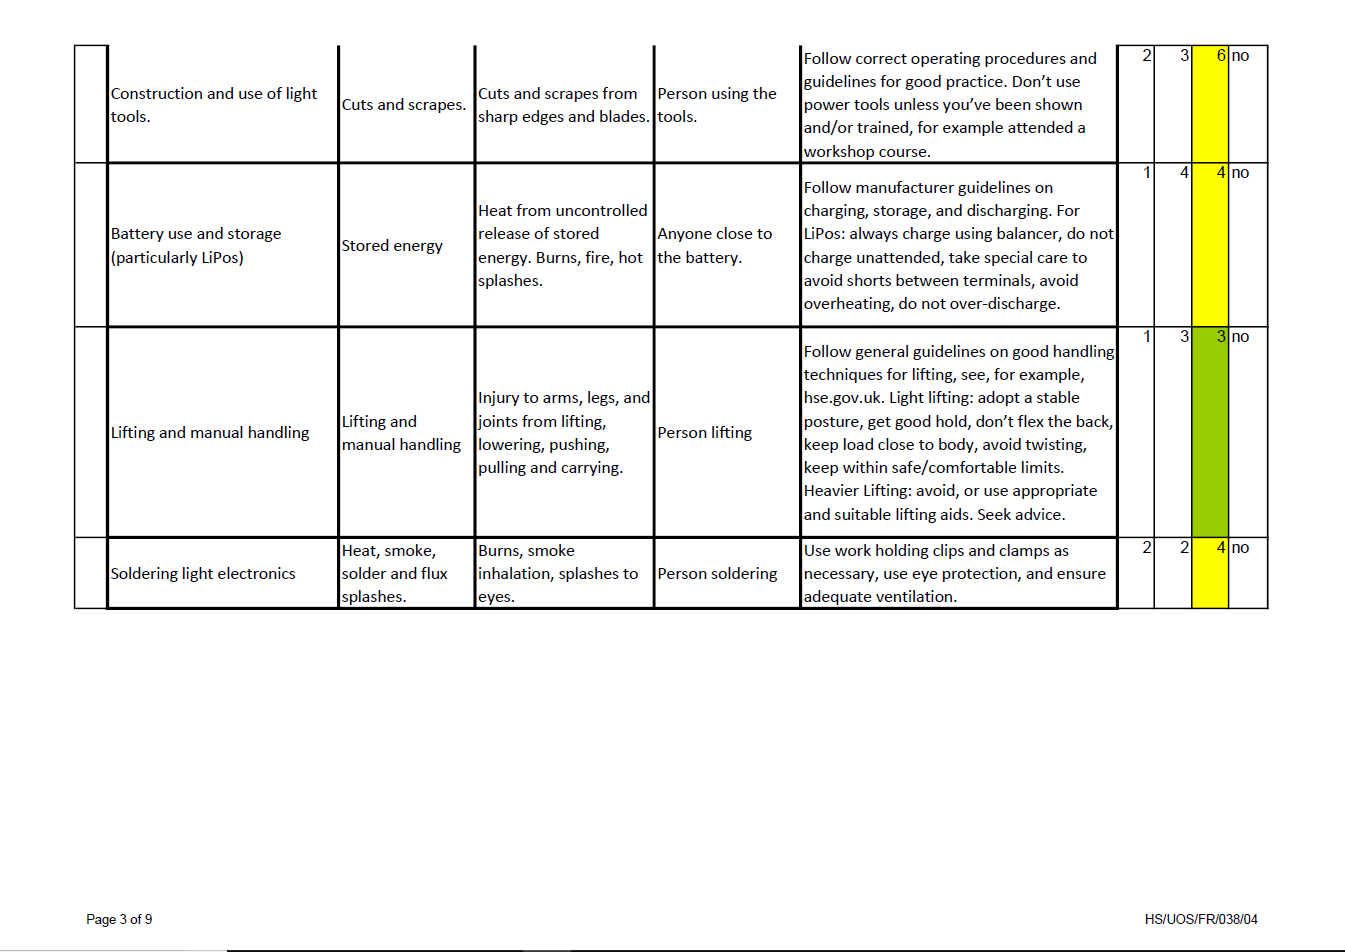
\includegraphics[scale=0.6]{ra3.png}
\caption{Section B}
\centering
\end{sidewaysfigure}
\newpage
\begin{sidewaysfigure}
\centering
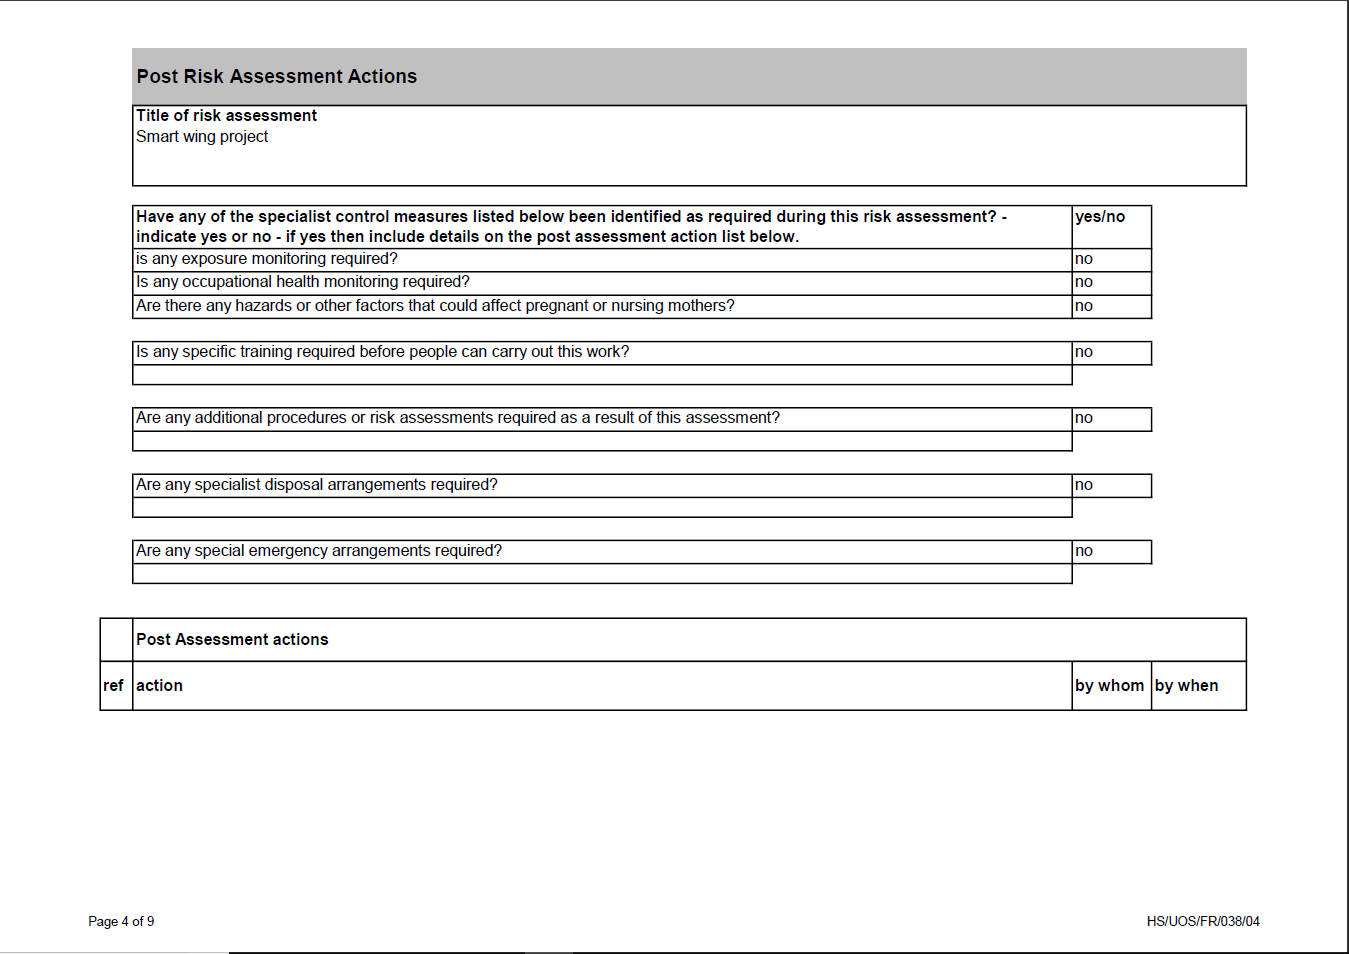
\includegraphics[scale=0.6]{ra4.png}
\caption{Section C}
\centering
\end{sidewaysfigure}

\chapter{Method Statement}
\thispagestyle{fancy}
This method statement is in reference to the project “Active Control of Wing Lift: Suppressing SPOs”. The scope of the work to be done is as follows: analysis of SPOs, design of controller, design of wing and the rig, building the wing, the rig and the gust generator and then finally testing the controller in a wind tunnel.
\newline
\newline
Most of the risk arises from manufacturing the parts and testing the controller in the wind tunnel. The wing will be split into four parts: the central section, the two ends of the wing and the movable trailing edge flap. The central section of the wing has pressure tappings which complicate the geometry of the part. 3D printing will therefore be necessary to produce this part. The ends of the wing are the same profile as the 3D printed parts. Due to the simple geometry of the part, the same profile can be laser cut several times and the laser cut parts can be stuck together side to side in order to extend the span of the wing. The flap will also be made similarly since all features of the flap are two dimensional. A RC servo will actuate the flap.
The wing will be mounted using some fixtures on the left and right walls of the wind tunnel. These are circular discs with holes in them for the carbon fibre rods and some more holes for the PVC tubes connected to the pressure tappings of the wing. These fixtures will be made exclusively by laser cutting.
\newline
\newline
The gust generator consists of two NACA0015 flaps which are 250mm in chord and 500mm in span. Due to the simple geometry, these can be foam cut. Laser cutting will be very inconvenient for this part due to the size of the flaps. The gust generator will operate by using two RC servos to deflect the flaps. Some carbon fibre rods will be used to provide structural support to the flaps. The rods will also serve as a shaft to connect the flap to the RC servos. The rods will be supported by a stand on either side of the flap as outlined in the diagram. These stands will be laser cut out of MDF.
\newline
\newline
Once the wing and gust generator is manufactured and mounted, the electronics need to be built. I will have to solder some differential pressure sensors onto a breadboard. These will be connected to a Raspberry Pi 3 (a microcontroller). The Raspberry Pi 3 will be connected to my laptop via WiFi through the Secure Shell protocol. This will allow me to monitor the data for my test. The Raspberry Pi will be running a code to implement my controller. It will use the pressure data to estimate the lift and remove the error by adjusting the flap angle through the RC servo mentioned above. The entire setup is outlined in the diagram on the next page.
\newline
\newline
The project will finish after testing the wing in the wind tunnel. I will use the Boldrewood wing tunnel (600mm by 400mm). I will firstly request induction and supervision from the lab supervisor. When testing, the wind tunnel will be turned on and the gust generator will be programmed to produce an impulsive gust by deflecting the flaps very quickly. The system should attempt to correct the lift change caused by the gust by moving the flap.
\begin{figure}[H]
\centering
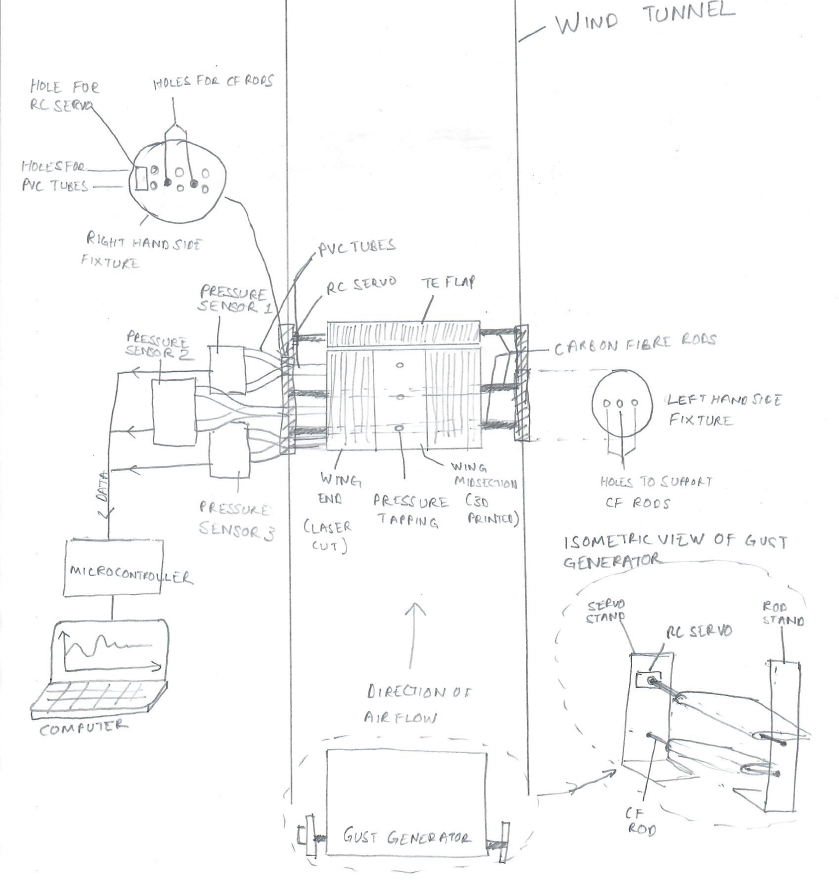
\includegraphics[scale=0.8]{msp.png}
\caption{Diagram of the setup}
\centering
\end{figure}
\chapter{Lift Estimator}
\thispagestyle{fancy}


\tiny
\begin{longtable}{|l|l|l|l|l|l|l|l|l|l|l|l|l|}
\caption{Lift estimator values and xfoil predicted values}
\label{tab:mylabel}
\tabularnewline
\hline
delta & alpha & Cp1     & Cp2     & Cp3     & p1       & p2       & p3       & Cl       & Actual Lift & Estimated Lift & Error\textasciicircum{}2 & \%Error     \\ \hline
0     & -5    & -0.5629 & -0.1619 & -0.0523 & -137.911 & -39.6655 & -12.8135 & -0.3757  & -2.485256   & -2.328769747   & 0.024488                 & 6.296565995 \\ \hline
0     & -4.5  & -0.4513 & -0.101  & -0.0122 & -110.569 & -24.745  & -2.989   & -0.3034  & -2.006991   & -1.84326134    & 0.026807                 & 8.157966835 \\ \hline
0     & -4    & -0.3476 & -0.0319 & 0.0351  & -85.162  & -7.8155  & 8.5995   & -0.223   & -1.475145   & -1.399489283   & 0.005724                 & 5.128696979 \\ \hline
0     & -3.5  & -0.3279 & 0.0311  & 0.0736  & -80.3355 & 7.6195   & 18.032   & -0.1551  & -1.025987   & -1.409230972   & 0.146876                 & 37.35375389 \\ \hline
0     & -3    & -0.2003 & 0.0998  & 0.1116  & -49.0735 & 24.451   & 27.342   & -0.0901  & -0.596012   & -0.897299727   & 0.090775                 & 50.55074051 \\ \hline
0     & -2.5  & -0.099  & 0.0947  & 0.1499  & -24.255  & 23.2015  & 36.7255  & -0.0306  & -0.202419   & -0.111006851   & 0.008356                 & 45.15986598 \\ \hline
0     & -2    & -0.01   & 0.1603  & 0.1742  & -2.45    & 39.2735  & 42.679   & 0.020367 & 0.1347255   & 0.134704751    & 4.31E-10                 & 0.01540107  \\ \hline
0     & -1.5  & 0.0744  & 0.2118  & 0.1779  & 18.228   & 51.891   & 43.5855  & 0.071333 & 0.47187     & 0.307820941    & 0.026912                 & 34.76573182 \\ \hline
0     & -1    & 0.1557  & 0.2578  & 0.2125  & 38.1465  & 63.161   & 52.0625  & 0.1223   & 0.8090145   & 0.685646144    & 0.01522                  & 15.24921447 \\ \hline
0     & -0.5  & 0.2402  & 0.3048  & 0.2465  & 58.849   & 74.676   & 60.3925  & 0.1734   & 1.147041    & 1.070744217    & 0.005821                 & 6.651617747 \\ \hline
0     & 0     & 0.3389  & 0.3626  & 0.2914  & 83.0305  & 88.837   & 71.393   & 0.2391   & 1.5816465   & 1.536447515    & 0.002043                 & 2.857717242 \\ \hline
0     & 0.5   & 0.4536  & 0.4322  & 0.3497  & 111.132  & 105.889  & 85.6765  & 0.3213   & 2.1253995   & 2.101900546    & 0.000552                 & 1.105625287 \\ \hline
0     & 1     & 0.5769  & 0.5086  & 0.417   & 141.3405 & 124.607  & 102.165  & 0.413    & 2.731995    & 2.729507842    & 6.19E-06                 & 0.091038158 \\ \hline
0     & 1.5   & 0.6637  & 0.5559  & 0.458   & 162.6065 & 136.1955 & 112.21   & 0.4685   & 3.0991275   & 3.167909238    & 0.004731                 & 2.219390401 \\ \hline
0     & 2     & 0.7423  & 0.5977  & 0.4959  & 181.8635 & 146.4365 & 121.4955 & 0.516    & 3.41334     & 3.575360908    & 0.026251                 & 4.746697009 \\ \hline
0     & 2.5   & 0.8211  & 0.641   & 0.5364  & 201.1695 & 157.045  & 131.418  & 0.5634   & 3.726891    & 3.991559243    & 0.070049                 & 7.101582601 \\ \hline
0     & 3     & 0.9001  & 0.6867  & 0.5217  & 220.5245 & 168.2415 & 127.8165 & 0.6109   & 4.0411035   & 4.055605192    & 0.00021                  & 0.358854756 \\ \hline
0     & 3.5   & 0.9791  & 0.7356  & 0.4583  & 239.8795 & 180.222  & 112.2835 & 0.6584   & 4.355316    & 3.802069646    & 0.306082                 & 12.70278331 \\ \hline
0     & 4     & 1.0583  & 0.7882  & 0.4727  & 259.2835 & 193.109  & 115.8115 & 0.7058   & 4.668867    & 4.008183434    & 0.436503                 & 14.15083286 \\ \hline
0     & 4.5   & 1.1376  & 0.8446  & 0.5056  & 278.712  & 206.927  & 123.872  & 0.753    & 4.981095    & 4.307719099    & 0.453435                 & 13.51863196 \\ \hline
0     & 5     & 1.2175  & 0.9047  & 0.5365  & 298.2875 & 221.6515 & 131.4425 & 0.8004   & 5.294646    & 4.577571966    & 0.514195                 & 13.54338013 \\ \hline
0     & 5.5   & 1.2981  & 0.9683  & 0.5642  & 318.0345 & 237.2335 & 138.229  & 0.8474   & 5.605551    & 4.811974158    & 0.629764                 & 14.15698193 \\ \hline
0     & 6     & 1.3801  & 0.9185  & 0.5891  & 338.1245 & 225.0325 & 144.3295 & 0.894    & 5.91381     & 5.663436156    & 0.062687                 & 4.233714715 \\ \hline
0     & 6.5   & 1.4644  & 0.9275  & 0.6113  & 358.778  & 227.2375 & 149.7685 & 0.9388   & 6.210162    & 6.184974825    & 0.000634                 & 0.405579992 \\ \hline
0     & 7     & 1.5562  & 0.9788  & 0.6301  & 381.269  & 239.806  & 154.3745 & 0.9809   & 6.4886535   & 6.490330372    & 2.81E-06                 & 0.025843141 \\ \hline
0     & 7.5   & 1.6219  & 1.0202  & 0.6452  & 397.3655 & 249.949  & 158.074  & 1.02     & 6.7473      & 6.693090432    & 0.002939                 & 0.803426084 \\ \hline
0     & 8     & 1.6171  & 1.0535  & 0.6567  & 396.1895 & 258.1075 & 160.8915 & 1.0566   & 6.989409    & 6.555015548    & 0.188698                 & 6.215024075 \\ \hline
0     & 8.5   & 1.6936  & 1.0822  & 0.6655  & 414.932  & 265.139  & 163.0475 & 1.0912   & 7.218288    & 6.844889064    & 0.139427                 & 5.172957019 \\ \hline
0     & 8     & 1.7583  & 1.1083  & 0.6721  & 430.7835 & 271.5335 & 164.6645 & 1.1245   & 7.4385675   & 7.07475877     & 0.132357                 & 4.890843973 \\ \hline
0     & 9.5   & 1.8145  & 1.1292  & 0.6737  & 444.5525 & 276.654  & 165.0565 & 1.1531   & 7.6277565   & 7.2587733      & 0.136149                 & 4.83737519  \\ \hline
0     & 10    & 2.1254  & 1.7566  & 1.7207  & 520.723  & 430.367  & 421.5715 & 1.1817   & 7.8169455   & 11.83941768    & 16.18028                 & 51.45836292 \\ \hline
15    & -5    & 0.4177  & 0.6491  & 0.7953  & 102.3365 & 159.0295 & 194.8485 & 0.728    & 4.81572     & 3.461323619    & 1.83439                  & 28.12448358 \\ \hline
15    & -4.5  & 0.5579  & 0.7427  & 0.8796  & 136.6855 & 181.9615 & 215.502  & 0.7856   & 5.196744    & 4.185627561    & 1.022356                 & 19.45672981 \\ \hline
15    & -4    & 0.7666  & 0.895   & 1.0023  & 187.817  & 219.275  & 245.5635 & 0.8432   & 5.577768    & 5.174937811    & 0.162272                 & 7.222067849 \\ \hline
15    & -3.5  & 0.8569  & 0.9405  & 1.0341  & 209.9405 & 230.4225 & 253.3545 & 0.9008   & 5.958792    & 5.584684986    & 0.139956                 & 6.278235821 \\ \hline
15    & -3    & 0.9472  & 0.9832  & 1.0652  & 232.064  & 240.884  & 260.974  & 0.9584   & 6.339816    & 6.005605243    & 0.111697                 & 5.271616034 \\ \hline
15    & -2.5  & 1.0045  & 1.0116  & 1.0731  & 246.1025 & 247.842  & 262.9095 & 0.9841   & 6.5098215   & 6.192611228    & 0.100622                 & 4.872795232 \\ \hline
15    & -2    & 1.0338  & 1.015   & 1.0337  & 253.281  & 248.675  & 253.2565 & 0.9804   & 6.485346    & 6.082245906    & 0.16249                  & 6.215552625 \\ \hline
15    & -1.5  & 1.0824  & 1.0342  & 1.0464  & 265.188  & 253.379  & 256.368  & 0.9971   & 6.5958165   & 6.304831666    & 0.084672                 & 4.411657513 \\ \hline
15    & -1    & 1.1377  & 1.0599  & 1.056   & 278.7365 & 259.6755 & 258.72   & 1.021    & 6.753915    & 6.506925645    & 0.061004                 & 3.656980506 \\ \hline
15    & -0.5  & 1.2023  & 1.0984  & 1.0691  & 294.5635 & 269.108  & 261.9295 & 1.054    & 6.97221     & 6.707735617    & 0.069947                 & 3.793264739 \\ \hline
15    & 0     & 1.2673  & 1.0869  & 1.0566  & 310.4885 & 266.2905 & 258.867  & 1.0864   & 7.186536    & 7.02945959     & 0.024673                 & 2.185704068 \\ \hline
15    & 0.5   & 1.3339  & 1.1346  & 1.0581  & 326.8055 & 277.977  & 259.2345 & 1.1218   & 7.420707    & 7.118275142    & 0.091465                 & 4.075512722 \\ \hline
15    & 1     & 1.4024  & 1.1728  & 1.0755  & 343.588  & 287.336  & 263.4975 & 1.1583   & 7.6621545   & 7.367328922    & 0.086922                 & 3.847815625 \\ \hline
15    & 1.5   & 1.4771  & 1.2083  & 1.0918  & 361.8895 & 296.0335 & 267.491  & 1.1952   & 7.906248    & 7.656503396    & 0.062372                 & 3.158825831 \\ \hline
15    & 2     & 1.5129  & 1.2449  & 1.1099  & 370.6605 & 305.0005 & 271.9255 & 1.2352   & 8.170848    & 7.75013252     & 0.177002                 & 5.148981838 \\ \hline
15    & 2.5   & 1.6046  & 1.2801  & 1.1276  & 393.127  & 313.6245 & 276.262  & 1.2757   & 8.4387555   & 8.137229375    & 0.090918                 & 3.573111281 \\ \hline
15    & 3     & 1.6818  & 1.3176  & 1.1455  & 412.041  & 322.812  & 280.6475 & 1.3177   & 8.7165855   & 8.438085282    & 0.077562                 & 3.195060935 \\ \hline
15    & 3.5   & 1.7543  & 1.3546  & 1.1633  & 429.8035 & 331.877  & 285.0085 & 1.3601   & 8.9970615   & 8.71685976     & 0.078513                 & 3.114369503 \\ \hline
15    & 4     & 1.8288  & 1.3906  & 1.1802  & 448.056  & 340.697  & 289.149  & 1.4026   & 9.278199    & 9.00593292     & 0.074129                 & 2.934471232 \\ \hline
15    & 4.5   & 1.9024  & 1.4263  & 1.1967  & 466.088  & 349.4435 & 293.1915 & 1.4451   & 9.5593365   & 9.289562006    & 0.072778                 & 2.822104797 \\ \hline
15    & 5     & 1.9747  & 1.462   & 1.2116  & 483.8015 & 358.19   & 296.842  & 1.4869   & 9.8358435   & 9.556636504    & 0.077957                 & 2.838668554 \\ \hline
15    & 5.5   & 2.0451  & 1.4971  & 1.2259  & 501.0495 & 366.7895 & 300.3455 & 1.5279   & 10.107059   & 9.813538877    & 0.086154                 & 2.904105316 \\ \hline
15    & 6     & 2.1167  & 1.5305  & 1.2389  & 518.5915 & 374.9725 & 303.5305 & 1.5684   & 10.374966   & 10.07802334    & 0.088175                 & 2.862107318 \\ \hline
15    & 6.5   & 2.1844  & 1.5625  & 1.2505  & 535.178  & 382.8125 & 306.3725 & 1.6073   & 10.63229    & 10.32152241    & 0.096576                 & 2.92286142  \\ \hline
15    & 7     & 2.2507  & 1.5934  & 1.2605  & 551.4215 & 390.383  & 308.8225 & 1.6454   & 10.884321   & 10.55403418    & 0.109089                 & 3.034519299 \\ \hline
15    & 7.5   & 2.3164  & 1.6236  & 1.2693  & 567.518  & 397.782  & 310.9785 & 1.6822   & 11.127753   & 10.77993418    & 0.120978                 & 3.125687794 \\ \hline
15    & 8     & 2.3806  & 1.6513  & 1.2764  & 583.247  & 404.5685 & 312.718  & 1.7176   & 11.361924   & 11.00145733    & 0.129936                 & 3.172584742 \\ \hline
15    & 8.5   & 2.4403  & 1.6774  & 1.2811  & 597.8735 & 410.963  & 313.8695 & 1.7509   & 11.582204   & 11.19384998    & 0.150818                 & 3.353019353 \\ \hline
15    & 9     & 2.4986  & 1.7021  & 1.2838  & 612.157  & 417.0145 & 314.531  & 1.7829   & 11.793884   & 11.37445113    & 0.175924                 & 3.556355003 \\ \hline
15    & 9.5   & 2.5559  & 1.7243  & 1.2848  & 626.1955 & 422.4535 & 314.776  & 1.8135   & 11.996303   & 11.55325316    & 0.196293                 & 3.693215816 \\ \hline
15    & 10    & 2.6103  & 1.7441  & 1.2826  & 639.5235 & 427.3045 & 314.237  & 1.8412   & 12.179538   & 11.71067099    & 0.219836                 & 3.849628825 \\ \hline
30    & -5    & 1.6576  & 1.6272  & 1.8181  & 406.112  & 398.664  & 445.4345 & 0.9964   & 6.591186    & 10.74303655    & 17.23786                 & 62.9909481  \\ \hline
30    & -4.5  & 1.5026  & 1.4945  & 1.6624  & 368.137  & 366.1525 & 407.288  & 1.0399   & 6.8789385   & 9.718980337    & 8.065838                 & 41.2860478  \\ \hline
30    & -4    & 1.4287  & 1.4285  & 1.5911  & 350.0315 & 349.9825 & 389.8195 & 1.0834   & 7.166691    & 9.263910112    & 4.398328                 & 29.26342313 \\ \hline
30    & -3.5  & 1.1681  & 1.1739  & 1.2518  & 286.1845 & 287.6055 & 306.691  & 1.1269   & 7.4544435   & 7.238950837    & 0.046437                 & 2.890794777 \\ \hline
30    & -3    & 1.2413  & 1.2164  & 1.2848  & 304.1185 & 298.018  & 314.776  & 1.1704   & 7.742196    & 7.584518907    & 0.024862                 & 2.036593916 \\ \hline
30    & -2.5  & 1.3197  & 1.2644  & 1.3101  & 323.3265 & 309.778  & 320.9745 & 1.2139   & 8.0299485   & 7.879065893    & 0.022766                 & 1.878998444 \\ \hline
30    & -2    & 1.4016  & 1.3162  & 1.3359  & 343.392  & 322.469  & 327.2955 & 1.2634   & 8.357391    & 8.173722429    & 0.033734                 & 2.197678335 \\ \hline
30    & -1.5  & 1.4808  & 1.3268  & 1.358   & 362.796  & 325.066  & 332.71   & 1.3091   & 8.6596965   & 8.659504826    & 3.67E-08                 & 0.002213403 \\ \hline
30    & -1    & 1.558   & 1.3779  & 1.3793  & 381.71   & 337.5855 & 337.9285 & 1.353    & 8.950095    & 8.906091479    & 0.001936                 & 0.491654229 \\ \hline
30    & -0.5  & 1.6451  & 1.4207  & 1.4018  & 403.0495 & 348.0715 & 343.441  & 1.398    & 9.24777     & 9.257004064    & 8.53E-05                 & 0.099851789 \\ \hline
30    & 0     & 1.6922  & 1.4636  & 1.424   & 414.589  & 358.582  & 348.88   & 1.4433   & 9.5474295   & 9.399298728    & 0.021943                 & 1.551525174 \\ \hline
30    & 0.5   & 1.7804  & 1.5014  & 1.4443  & 436.198  & 367.843  & 353.8535 & 1.4861   & 9.8305515   & 9.769984295    & 0.003668                 & 0.616111975 \\ \hline
30    & 1     & 1.856   & 1.54    & 1.4631  & 454.72   & 377.3    & 358.4595 & 1.5282   & 10.109043   & 10.06205071    & 0.002208                 & 0.464853965 \\ \hline
30    & 1.5   & 1.9291  & 1.5774  & 1.4778  & 472.6295 & 386.463  & 362.061  & 1.5701   & 10.386212   & 10.32261727    & 0.004044                 & 0.612294813 \\ \hline
30    & 2     & 2.0044  & 1.6137  & 1.4835  & 491.078  & 395.3565 & 363.4575 & 1.6116   & 10.660734   & 10.5451882     & 0.013351                 & 1.08384468  \\ \hline
30    & 2.5   & 2.0787  & 1.6495  & 1.467   & 509.2815 & 404.1275 & 359.415  & 1.6526   & 10.931949   & 10.62866494    & 0.091981                 & 2.774290851 \\ \hline
30    & 3     & 2.1499  & 1.6842  & 1.4779  & 526.7255 & 412.629  & 362.0855 & 1.6925   & 11.195888   & 10.870967      & 0.105573                 & 2.902141511 \\ \hline
30    & 3.5   & 2.2209  & 1.7179  & 1.493   & 544.1205 & 420.8855 & 365.785  & 1.7315   & 11.453873   & 11.14363068    & 0.09625                  & 2.708619499 \\ \hline
30    & 4     & 2.2893  & 1.7496  & 1.5061  & 560.8785 & 428.652  & 368.9945 & 1.7692   & 11.703258   & 11.40163424    & 0.090977                 & 2.577263144 \\ \hline
30    & 4.5   & 2.3546  & 1.7811  & 1.5179  & 576.877  & 436.3695 & 371.8855 & 1.8057   & 11.944706   & 11.63675675    & 0.094832                 & 2.578119246 \\ \hline
30    & 5     & 2.421   & 1.81    & 1.5278  & 593.145  & 443.45   & 374.311  & 1.8409   & 12.177554   & 11.88022796    & 0.088402                 & 2.441586801 \\ \hline
30    & 5.5   & 2.4823  & 1.8377  & 1.5357  & 608.1635 & 450.2365 & 376.2465 & 1.8746   & 12.400479   & 12.09172659    & 0.095328                 & 2.489842574 \\ \hline
30    & 6     & 2.5465  & 1.863   & 1.5406  & 623.8925 & 456.435  & 377.447  & 1.906    & 12.60819    & 12.31297415    & 0.087152                 & 2.341460955 \\ \hline
30    & 6.5   & 2.6051  & 1.8871  & 1.5447  & 638.2495 & 462.3395 & 378.4515 & 1.9371   & 12.813917   & 12.5070608     & 0.09416                  & 2.394706545 \\ \hline
30    & 7     & 2.662   & 1.9092  & 1.5449  & 652.19   & 467.754  & 378.5005 & 1.9654   & 13.001121   & 12.67942738    & 0.103487                 & 2.474352964 \\ \hline
30    & 7.5   & 2.7149  & 1.9276  & 1.5407  & 665.1505 & 472.262  & 377.4715 & 1.9903   & 13.165835   & 12.82453819    & 0.116483                 & 2.592287748 \\ \hline
30    & 8     & 2.7652  & 1.9429  & 1.5336  & 677.474  & 476.0105 & 375.732  & 2.0132   & 13.317318   & 12.95552967    & 0.130891                 & 2.716675588 \\ \hline
30    & 8.5   & 2.8135  & 1.9586  & 1.5265  & 689.3075 & 479.857  & 373.9925 & 2.0367   & 13.472771   & 13.07399834    & 0.159019                 & 2.959837814 \\ \hline
30    & 9     & 2.8571  & 1.969   & 1.5121  & 699.9895 & 482.405  & 370.4645 & 2.055    & 13.593825   & 13.1525925     & 0.194686                 & 3.245830361 \\ \hline
30    & 9.5   & 2.8951  & 1.975   & 1.4924  & 709.2995 & 483.875  & 365.638  & 2.0698   & 13.691727   & 13.19401104    & 0.247721                 & 3.635158396 \\ \hline
30    & 10    & 2.935   & 1.982   & 1.474   & 719.075  & 485.59   & 361.13   & 2.0867   & 13.803521   & 13.24770024    & 0.308936                 & 4.02665584  \\ \hline
45    & -5    & 2.0434  & 1.952   & 2.1479  & 500.633  & 478.24   & 526.2355 & 1.3171   & 8.7126165   & 12.96676264    & 18.09776                 & 48.82742333 \\ \hline
45    & -4.5  & 1.9784  & 1.8978  & 2.0908  & 484.708  & 464.961  & 512.246  & 1.3595   & 8.9930925   & 12.57976479    & 12.86422                 & 39.88252412 \\ \hline
45    & -4    & 1.9245  & 1.8549  & 2.0427  & 471.5025 & 454.4505 & 500.4615 & 1.4019   & 9.2735685   & 12.2429255     & 8.817081                 & 32.01957266 \\ \hline
45    & -3.5  & 1.888   & 1.8055  & 1.9825  & 462.56   & 442.3475 & 485.7125 & 1.4443   & 9.5540445   & 11.95722519    & 5.775277                 & 25.15354293 \\ \hline
45    & -3    & 1.834   & 1.7343  & 1.8848  & 449.33   & 424.9035 & 461.776  & 1.4867   & 9.8345205   & 11.47093685    & 2.677858                 & 16.63951334 \\ \hline
45    & -2.5  & 1.7773  & 1.6115  & 1.6686  & 435.4385 & 394.8175 & 408.807  & 1.5291   & 10.114997   & 10.52636661    & 0.169225                 & 4.066932771 \\ \hline
45    & -2    & 1.8208  & 1.6509  & 1.6843  & 446.096  & 404.4705 & 412.6535 & 1.5715   & 10.395473   & 10.62943028    & 0.054736                 & 2.250573832 \\ \hline
45    & -1.5  & 1.9057  & 1.6898  & 1.6993  & 466.8965 & 414.001  & 416.3285 & 1.6134   & 10.672641   & 10.94438361    & 0.073844                 & 2.546160874 \\ \hline
45    & -1    & 1.9805  & 1.7271  & 1.7121  & 485.2225 & 423.1395 & 419.4645 & 1.6533   & 10.93658    & 11.20256753    & 0.07075                  & 2.432095241 \\ \hline
45    & -0.5  & 2.053   & 1.7623  & 1.7236  & 502.985  & 431.7635 & 422.282  & 1.6921   & 11.193242   & 11.45250144    & 0.067216                 & 2.316218554 \\ \hline
45    & 0     & 2.1234  & 1.7959  & 1.7339  & 520.233  & 439.9955 & 424.8055 & 1.7298   & 11.442627   & 11.69306728    & 0.06272                  & 2.188660691 \\ \hline
45    & 0.5   & 2.1931  & 1.8287  & 1.7432  & 537.3095 & 448.0315 & 427.084  & 1.7667   & 11.686721   & 11.92829036    & 0.058356                 & 2.067045792 \\ \hline
45    & 1     & 2.2619  & 1.8599  & 1.7518  & 554.1655 & 455.6755 & 429.191  & 1.8024   & 11.922876   & 12.16341082    & 0.057857                 & 2.01742285  \\ \hline
45    & 1.5   & 2.3277  & 1.8892  & 1.7583  & 570.2865 & 462.854  & 430.7835 & 1.8368   & 12.150432   & 12.38064024    & 0.052996                 & 1.894650634 \\ \hline
45    & 2     & 2.3917  & 1.9186  & 1.7633  & 585.9665 & 470.057  & 432.0085 & 1.8696   & 12.367404   & 12.57880014    & 0.044688                 & 1.709300821 \\ \hline
45    & 2.5   & 2.4531  & 1.9445  & 1.7658  & 601.0095 & 476.4025 & 432.621  & 1.9004   & 12.571146   & 12.76751578    & 0.038561                 & 1.562067492 \\ \hline
45    & 3     & 2.5151  & 1.9691  & 1.767   & 616.1995 & 482.4295 & 432.915  & 1.9301   & 12.767612   & 12.95850832    & 0.036442                 & 1.495164698 \\ \hline
45    & 3.5   & 2.5735  & 1.9917  & 1.7668  & 630.5075 & 487.9665 & 432.866  & 1.9583   & 12.954155   & 13.13338       & 0.032122                 & 1.383536867 \\ \hline
45    & 4     & 2.63    & 2.0135  & 1.764   & 644.35   & 493.3075 & 432.18   & 1.9851   & 13.131437   & 13.28686988    & 0.02416                  & 1.183673882 \\ \hline
45    & 4.5   & 2.6848  & 2.0334  & 1.7597  & 657.776  & 498.183  & 431.1265 & 2.0104   & 13.298796   & 13.43286548    & 0.017975                 & 1.008132482 \\ \hline
45    & 5     & 2.7338  & 2.0494  & 1.7494  & 669.781  & 502.103  & 428.603  & 2.0317   & 13.439696   & 13.53357897    & 0.008814                 & 0.698553577 \\ \hline
45    & 5.5   & 2.7862  & 2.0646  & 1.7386  & 682.619  & 505.827  & 425.957  & 2.0538   & 13.585887   & 13.65316592    & 0.004526                 & 0.495211849 \\ \hline
45    & 6     & 2.8305  & 2.0742  & 1.7189  & 693.4725 & 508.179  & 421.1305 & 2.0706   & 13.697019   & 13.7071563     & 0.000103                 & 0.074010968 \\ \hline
45    & 6.5   & 2.8754  & 2.0863  & 1.6969  & 704.473  & 511.1435 & 415.7405 & 2.0896   & 13.822704   & 13.73625234    & 0.007474                 & 0.625432367 \\ \hline
45    & 7     & 2.9151  & 2.0924  & 1.6674  & 714.1995 & 512.638  & 408.513  & 2.104    & 13.91796    & 13.72553546    & 0.037027                 & 1.382562786 \\ \hline
45    & 7.5   & 2.9506  & 2.0948  & 1.6262  & 722.897  & 513.226  & 398.419  & 2.1152   & 13.992048   & 13.64157963    & 0.122828                 & 2.504768216 \\ \hline
45    & 8     & 2.9859  & 2.0968  & 1.5853  & 731.5455 & 513.716  & 388.3985 & 2.1275   & 14.073413   & 13.56065199    & 0.262923                 & 3.643469634 \\ \hline
45    & 8.5   & 3.0167  & 2.0946  & 1.5436  & 739.0915 & 513.177  & 378.182  & 2.1367   & 14.134271   & 13.47482395    & 0.43487                  & 4.665586039 \\ \hline
45    & 9     & 3.038   & 2.0853  & 1.4983  & 744.31   & 510.8985 & 367.0835 & 2.1408   & 14.161392   & 13.35711295    & 0.646865                 & 5.679378512 \\ \hline
45    & 9.5   & 3.0624  & 2.0738  & 1.4491  & 750.288  & 508.081  & 355.0295 & 2.1453   & 14.19116    & 13.24353395    & 0.897994                 & 6.677576647 \\ \hline
45    & 10    & 3.0852  & 2.0613  & 1.3962  & 755.874  & 505.0185 & 342.069  & 2.1502   & 14.223573   & 13.10445214    & 1.252431                 & 7.86807126  \\ \hline
60    & -5    & 2.8981  & 2.6236  & 2.7989  & 710.0345 & 642.782  & 685.7305 & 1.5257   & 10.092506   & 17.66801805    & 57.38839                 & 75.06077212 \\ \hline
60    & -4.5  & 2.0694  & 1.9289  & 2.0895  & 507.003  & 472.5805 & 511.9275 & 1.5613   & 10.328      & 12.86892654    & 6.45631                  & 24.60231568 \\ \hline
60    & -4    & 2.0209  & 1.8818  & 2.031   & 495.1205 & 461.041  & 497.595  & 1.5969   & 10.563494   & 12.51911061    & 3.824438                 & 18.51297686 \\ \hline
60    & -3.5  & 1.9676  & 1.8034  & 1.9045  & 482.062  & 441.833  & 466.6025 & 1.6325   & 10.798988   & 11.89890063    & 1.209809                 & 10.1853357  \\ \hline
60    & -3    & 2.0345  & 1.8354  & 1.9131  & 498.4525 & 449.673  & 468.7095 & 1.6681   & 11.034482   & 12.11980188    & 1.17792                  & 9.83571707  \\ \hline
60    & -2.5  & 2.104   & 1.87    & 1.9244  & 515.48   & 458.15   & 471.478  & 1.7037   & 11.269976   & 12.35635581    & 1.180222                 & 9.639597786 \\ \hline
60    & -2    & 2.1718  & 1.904   & 1.9321  & 532.091  & 466.48   & 473.3645 & 1.7384   & 11.499516   & 12.56529523    & 1.135885                 & 9.268035546 \\ \hline
60    & -1.5  & 2.2379  & 1.936   & 1.9377  & 548.2855 & 474.32   & 474.7365 & 1.7721   & 11.722442   & 12.76359866    & 1.084008                 & 8.881743276 \\ \hline
60    & -1    & 2.3036  & 1.9658  & 1.9405  & 564.382  & 481.621  & 475.4225 & 1.8029   & 11.926184   & 12.95476366    & 1.057977                 & 8.624554202 \\ \hline
60    & -0.5  & 2.3633  & 1.9935  & 1.9401  & 579.0085 & 488.4075 & 475.3245 & 1.8328   & 12.123972   & 13.10690366    & 0.966155                 & 8.107340199 \\ \hline
60    & 0     & 2.4253  & 2.0194  & 1.9376  & 594.1985 & 494.753  & 474.712  & 1.8645   & 12.333668   & 13.26792345    & 0.872834                 & 7.574843    \\ \hline
60    & 0.5   & 2.485   & 2.0432  & 1.9348  & 608.825  & 500.584  & 474.026  & 1.8926   & 12.519549   & 13.42685105    & 0.823197                 & 7.247082566 \\ \hline
60    & 1     & 2.5439  & 2.0664  & 1.9303  & 623.2555 & 506.268  & 472.9235 & 1.9198   & 12.699477   & 13.57450391    & 0.765672                 & 6.89025942  \\ \hline
60    & 1.5   & 2.5991  & 2.0871  & 1.9226  & 636.7795 & 511.3395 & 471.037  & 1.9463   & 12.874775   & 13.69720121    & 0.676386                 & 6.38789216  \\ \hline
60    & 2     & 2.6515  & 2.1055  & 1.9118  & 649.6175 & 515.8475 & 468.391  & 1.9693   & 13.02692    & 13.79909266    & 0.596251                 & 5.927519278 \\ \hline
60    & 2.5   & 2.7039  & 2.1223  & 1.9     & 662.4555 & 519.9635 & 465.5    & 1.9915   & 13.173773   & 13.90367404    & 0.532756                 & 5.540565866 \\ \hline
60    & 3     & 2.7536  & 2.138   & 1.8838  & 674.632  & 523.81   & 461.531  & 2.0136   & 13.319964   & 13.97332414    & 0.426879                 & 4.905119384 \\ \hline
60    & 3.5   & 2.8005  & 2.1498  & 1.8686  & 686.1225 & 526.701  & 457.807  & 2.0317   & 13.439696   & 14.05626321    & 0.380156                 & 4.587661277 \\ \hline
60    & 4     & 2.8472  & 2.1607  & 1.8466  & 697.564  & 529.3715 & 452.417  & 2.0504   & 13.563396   & 14.10127485    & 0.289314                 & 3.965664994 \\ \hline
60    & 4.5   & 2.8864  & 2.1679  & 1.8244  & 707.168  & 531.1355 & 446.978  & 2.0652   & 13.661298   & 14.12684954    & 0.216738                 & 3.407813381 \\ \hline
60    & 5     & 2.9289  & 2.175   & 1.796   & 717.5805 & 532.875  & 440.02   & 2.081    & 13.765815   & 14.13181167    & 0.133954                 & 2.658735901 \\ \hline
60    & 5.5   & 2.9654  & 2.1775  & 1.7661  & 726.523  & 533.4875 & 432.6945 & 2.0929   & 13.844534   & 14.12204169    & 0.077011                 & 2.004460388 \\ \hline
60    & 6     & 2.9975  & 2.176   & 1.7282  & 734.3875 & 533.12   & 423.409  & 2.1026   & 13.908699   & 14.06244456    & 0.023638                 & 1.105391387 \\ \hline
60    & 6.5   & 3.0307  & 2.1759  & 1.6877  & 742.5215 & 533.0955 & 413.4865 & 2.1138   & 13.982787   & 13.9847663     & 3.92E-06                 & 0.014155228 \\ \hline
60    & 7     & 3.0584  & 2.1706  & 1.6434  & 749.308  & 531.797  & 402.633  & 2.122    & 14.03703    & 13.88408856    & 0.023391                 & 1.089556968 \\ \hline
60    & 7.5   & 3.0848  & 2.1614  & 1.59    & 755.776  & 529.543  & 389.55   & 2.1282   & 14.078043   & 13.74223895    & 0.112764                 & 2.385303502 \\ \hline
60    & 8     & 3.102   & 2.1449  & 1.5254  & 759.99   & 525.5005 & 373.723  & 2.1306   & 14.093919   & 13.52435951    & 0.324398                 & 4.041171851 \\ \hline
60    & 8.5   & 3.1239  & 2.1291  & 1.4662  & 765.3555 & 521.6295 & 359.219  & 2.1348   & 14.121702   & 13.360092      & 0.58005                  & 5.393188429 \\ \hline
60    & 9     & 3.1387  & 2.1082  & 1.404   & 768.9815 & 516.509  & 343.98   & 2.1372   & 14.137578   & 13.16894959    & 0.938241                 & 6.851445182 \\ \hline
60    & 9.5   & 3.1515  & 2.0817  & 1.344   & 772.1175 & 510.0165 & 329.28   & 2.1387   & 14.147501   & 13.01201063    & 1.289337                 & 8.026081125 \\ \hline
60    & 10    & 3.1578  & 2.047   & 1.3008  & 773.661  & 501.515  & 318.696  & 2.1367   & 14.134271   & 12.97035745    & 1.354694                 & 8.234687791 \\ \hline
-15   & -5    & -1.5325 & -0.9498 & -0.8876 & -375.463 & -232.701 & -217.462 & -1.2972  & -8.580978   & -8.114151402   & 0.217927                 & 5.440249328 \\ \hline
-15   & -4.5  & -1.4534 & -0.9063 & -0.8626 & -356.083 & -222.044 & -211.337 & -1.245   & -8.235675   & -7.792958666   & 0.195998                 & 5.375592573 \\ \hline
-15   & -4    & -1.3735 & -0.8624 & -0.8371 & -336.508 & -211.288 & -205.09  & -1.1924  & -7.887726   & -7.466774604   & 0.1772                   & 5.336790298 \\ \hline
-15   & -3.5  & -1.2929 & -0.8183 & -0.8121 & -316.761 & -200.484 & -198.965 & -1.1396  & -7.538454   & -7.141166614   & 0.157837                 & 5.270144062 \\ \hline
-15   & -3    & -1.212  & -0.7733 & -0.7867 & -296.94  & -189.459 & -192.742 & -1.0865  & -7.187198   & -6.816525721   & 0.137398                 & 5.157389638 \\ \hline
-15   & -2.5  & -1.131  & -0.7287 & -0.761  & -277.095 & -178.532 & -186.445 & -1.0333  & -6.83528    & -6.48731       & 0.121083                 & 5.090786709 \\ \hline
-15   & -2    & -1.0478 & -0.6837 & -0.7353 & -256.711 & -167.507 & -180.149 & -0.9798  & -6.481377   & -6.148964248   & 0.110498                 & 5.128736564 \\ \hline
-15   & -1.5  & -0.9662 & -0.6381 & -0.7095 & -236.719 & -156.335 & -173.828 & -0.9263  & -6.127475   & -5.821569323   & 0.093578                 & 4.99235333  \\ \hline
-15   & -1    & -0.8834 & -0.5924 & -0.6832 & -216.433 & -145.138 & -167.384 & -0.8724  & -5.770926   & -5.485461942   & 0.08149                  & 4.94659016  \\ \hline
-15   & -0.5  & -0.8007 & -0.5459 & -0.6569 & -196.172 & -133.746 & -160.941 & -0.8186  & -5.415039   & -5.15429398    & 0.067988                 & 4.815201153 \\ \hline
-15   & 0     & -0.7158 & -0.4991 & -0.6304 & -175.371 & -122.28  & -154.448 & -0.7645  & -5.057168   & -4.812211437   & 0.060003                 & 4.843740345 \\ \hline
-15   & 0.5   & -0.633  & -0.4481 & -0.6039 & -155.085 & -109.785 & -147.956 & -0.7105  & -4.699958   & -4.504180656   & 0.038329                 & 4.165502441 \\ \hline
-15   & 1     & -0.5488 & -0.4199 & -0.5768 & -134.456 & -102.876 & -141.316 & -0.6558  & -4.338117   & -4.059157164   & 0.077819                 & 6.430435974 \\ \hline
-15   & 1.5   & -0.463  & -0.3702 & -0.5498 & -113.435 & -90.699  & -134.701 & -0.601   & -3.975615   & -3.725392356   & 0.062611                 & 6.293935496 \\ \hline
-15   & 2     & -0.379  & -0.3189 & -0.5225 & -92.855  & -78.1305 & -128.013 & -0.5461  & -3.612452   & -3.407907741   & 0.041838                 & 5.662187002 \\ \hline
-15   & 2.5   & -0.2943 & -0.2702 & -0.4952 & -72.1035 & -66.199  & -121.324 & -0.4914  & -3.250611   & -3.072436728   & 0.031746                 & 5.481254823 \\ \hline
-15   & 3     & -0.2083 & -0.2228 & -0.4677 & -51.0335 & -54.586  & -114.587 & -0.4362  & -2.885463   & -2.721843284   & 0.026771                 & 5.670483948 \\ \hline
-15   & 3.5   & -0.1226 & -0.1757 & -0.4404 & -30.037  & -43.0465 & -107.898 & -0.3812  & -2.521638   & -2.372369084   & 0.022281                 & 5.919522005 \\ \hline
-15   & 4     & -0.0371 & -0.1276 & -0.4126 & -9.0895  & -31.262  & -101.087 & -0.3258  & -2.155167   & -2.026376902   & 0.016587                 & 5.975875558 \\ \hline
-15   & 4.5   & 0.0487  & -0.08   & -0.3853 & 11.9315  & -19.6    & -94.3985 & -0.2707  & -1.790681   & -1.679152079   & 0.012439                 & 6.228270255 \\ \hline
-15   & 5     & 0.1348  & -0.0325 & -0.3572 & 33.026   & -7.9625  & -87.514  & -0.2149  & -1.421564   & -1.324901381   & 0.009344                 & 6.799704605 \\ \hline
-15   & 5.5   & 0.2346  & 0.0157  & -0.3291 & 57.477   & 3.8465   & -80.6295 & -0.1588  & -1.050462   & -0.903892049   & 0.021483                 & 13.95290371 \\ \hline
-15   & 6     & 0.2959  & 0.0635  & -0.3007 & 72.4955  & 15.5575  & -73.6715 & -0.1024  & -0.677376   & -0.677307862   & 4.64E-09                 & 0.010059167 \\ \hline
-15   & 6.5   & 0.3864  & 0.1113  & -0.2729 & 94.668   & 27.2685  & -66.8605 & -0.0461  & -0.304952   & -0.303879529   & 1.15E-06                 & 0.351521911 \\ \hline
-15   & 7     & 0.4761  & 0.1578  & -0.2443 & 116.6445 & 38.661   & -59.8535 & 0.0102   & 0.067473    & 0.077539506    & 0.000101                 & 14.91930995 \\ \hline
-15   & 7.5   & 0.5618  & 0.2072  & -0.2165 & 137.641  & 50.764   & -53.0425 & 0.066    & 0.43659     & 0.417373981    & 0.000369                 & 4.401387826 \\ \hline
-15   & 8     & 0.6458  & 0.2619  & -0.188  & 158.221  & 64.1655  & -46.06   & 0.12255  & 0.8106683   & 0.723446521    & 0.007608                 & 10.75923827 \\ \hline
-15   & 8.5   & 0.7319  & 0.3011  & -0.1599 & 179.3155 & 73.7695  & -39.1755 & 0.1791   & 1.1847465   & 1.123594909    & 0.00374                  & 5.161576015 \\ \hline
-15   & 9     & 0.816   & 0.3466  & -0.1312 & 199.92   & 84.917   & -32.144  & 0.23565  & 1.5588248   & 1.482289105    & 0.005858                 & 4.909829955 \\ \hline
-15   & 9.5   & 0.9018  & 0.394   & -0.1008 & 220.941  & 96.53    & -24.696  & 0.2922   & 1.932903    & 1.849709149    & 0.006921                 & 4.304088231 \\ \hline
-15   & 10    & 0.9354  & 0.4119  & -0.0862 & 229.173  & 100.9155 & -21.119  & 0.34875  & 2.3069813   & 2.013851972    & 0.085925                 & 12.7061838  \\ \hline
-30   & -5    & -2.0184 & -1.3441 & -1.3023 & -494.508 & -329.305 & -319.064 & -1.7167  & -11.35597   & -10.99241219   & 0.132175                 & 3.201472836 \\ \hline
-30   & -4.5  & -1.9454 & -1.3052 & -1.2828 & -476.623 & -319.774 & -314.286 & -1.6698  & -11.04573   & -10.71109839   & 0.111976                 & 3.029484696 \\ \hline
-30   & -4    & -1.872  & -1.2659 & -1.263  & -458.64  & -310.146 & -309.435 & -1.6229  & -10.73548   & -10.42808701   & 0.094493                 & 2.863368877 \\ \hline
-30   & -3.5  & -1.7979 & -1.2275 & -1.2431 & -440.486 & -300.738 & -304.56  & -1.5757  & -10.42326   & -10.13587417   & 0.082588                 & 2.757116773 \\ \hline
-30   & -3    & -1.7215 & -1.1858 & -1.2216 & -421.768 & -290.521 & -299.292 & -1.5269  & -10.10044   & -9.840199792   & 0.067727                 & 2.576557236 \\ \hline
-30   & -2.5  & -1.6461 & -1.145  & -1.1999 & -403.295 & -280.525 & -293.976 & -1.4782  & -9.778293   & -9.543472427   & 0.055141                 & 2.401447502 \\ \hline
-30   & -2    & -1.5689 & -1.1042 & -1.1786 & -384.381 & -270.529 & -288.757 & -1.4299  & -9.458789   & -9.2399284     & 0.0479                   & 2.313828036 \\ \hline
-30   & -1.5  & -1.4924 & -1.0634 & -1.1573 & -365.638 & -260.533 & -283.539 & -1.3818  & -9.140607   & -8.93999318    & 0.040246                 & 2.194753801 \\ \hline
-30   & -1    & -1.415  & -1.0218 & -1.1361 & -346.675 & -250.341 & -278.345 & -1.3335  & -8.821103   & -8.640457721   & 0.032633                 & 2.047870759 \\ \hline
-30   & -0.5  & -1.339  & -0.9805 & -1.1145 & -328.055 & -240.223 & -273.053 & -1.285   & -8.500275   & -8.344017796   & 0.024416                 & 1.838260577 \\ \hline
-30   & 0     & -1.2584 & -0.9372 & -1.0908 & -308.308 & -229.614 & -267.246 & -1.2347  & -8.167541   & -8.021991103   & 0.021185                 & 1.78204684  \\ \hline
-30   & 0.5   & -1.1805 & -0.8949 & -1.0677 & -289.223 & -219.251 & -261.587 & -1.1852  & -7.840098   & -7.712048949   & 0.016397                 & 1.633258301 \\ \hline
-30   & 1     & -1.1016 & -0.8513 & -1.0457 & -269.892 & -208.569 & -256.197 & -1.1363  & -7.516625   & -7.410913755   & 0.011175                 & 1.406359259 \\ \hline
-30   & 1.5   & -1.0242 & -0.8036 & -1.0235 & -250.929 & -196.882 & -250.758 & -1.0874  & -7.193151   & -7.13895251    & 0.002937                 & 0.753473551 \\ \hline
-30   & 2     & -0.9441 & -0.7787 & -1.0012 & -231.305 & -190.782 & -245.294 & -1.0386  & -6.870339   & -6.726375394   & 0.020726                 & 2.095436713 \\ \hline
-30   & 2.5   & -0.8656 & -0.7334 & -0.9789 & -212.072 & -179.683 & -239.831 & -0.9895  & -6.545543   & -6.434855762   & 0.012252                 & 1.69102467  \\ \hline
-30   & 3     & -0.7838 & -0.6876 & -0.9546 & -192.031 & -168.462 & -233.877 & -0.9387  & -6.209501   & -6.116772452   & 0.008598                 & 1.493325399 \\ \hline
-30   & 3.5   & -0.7044 & -0.6417 & -0.9301 & -172.578 & -157.217 & -227.875 & -0.8877  & -5.872136   & -5.810383617   & 0.003813                 & 1.051608616 \\ \hline
-30   & 4     & -0.6242 & -0.5986 & -0.9071 & -152.929 & -146.657 & -222.24  & -0.838   & -5.54337    & -5.493623608   & 0.002475                 & 0.897403424 \\ \hline
-30   & 4.5   & -0.5446 & -0.5546 & -0.8847 & -133.427 & -135.877 & -216.752 & -0.7887  & -5.217251   & -5.188628414   & 0.000819                 & 0.548604782 \\ \hline
-30   & 5     & -0.4662 & -0.5122 & -0.8618 & -114.219 & -125.489 & -211.141 & -0.7393  & -4.89047    & -4.877893089   & 0.000158                 & 0.257161622 \\ \hline
-30   & 5.5   & -0.3855 & -0.4692 & -0.8392 & -94.4475 & -114.954 & -205.604 & -0.6899  & -4.563689   & -4.560465505   & 1.04E-05                 & 0.070622584 \\ \hline
-30   & 6     & -0.3047 & -0.4257 & -0.8158 & -74.6515 & -104.297 & -199.871 & -0.6369  & -4.213094   & -4.24036104    & 0.000744                 & 0.647209458 \\ \hline
-30   & 6.5   & -0.2185 & -0.3788 & -0.7882 & -53.5325 & -92.806  & -193.109 & -0.5839  & -3.862499   & -3.885355804   & 0.000522                 & 0.591775097 \\ \hline
-30   & 7     & -0.1375 & -0.3351 & -0.7649 & -33.6875 & -82.0995 & -187.401 & -0.5336  & -3.529764   & -3.565942001   & 0.001309                 & 1.024941083 \\ \hline
-30   & 7.5   & -0.0659 & -0.2908 & -0.7422 & -16.1455 & -71.246  & -181.839 & -0.4829  & -3.194384   & -3.302001931   & 0.011582                 & 3.368989078 \\ \hline
-30   & 8     & 0.0194  & -0.2501 & -0.7204 & 4.753    & -61.2745 & -176.498 & -0.4334  & -2.866941   & -2.953066946   & 0.007418                 & 3.004105991 \\ \hline
-30   & 8.5   & 0.0973  & -0.2066 & -0.6972 & 23.8385  & -50.617  & -170.814 & -0.3839  & -2.539499   & -2.649144821   & 0.012022                 & 4.317636751 \\ \hline
-30   & 9     & 0.1794  & -0.1617 & -0.6737 & 43.953   & -39.6165 & -165.057 & -0.32767 & -2.167515   & -2.32946428    & 0.026228                 & 7.471656705 \\ \hline
-30   & 9.5   & 0.2929  & -0.0923 & -0.6216 & 71.7605  & -22.6135 & -152.292 & -0.27143 & -1.795532   & -1.807270314   & 0.000138                 & 0.653779332 \\ \hline
-30   & 10    & 0.3548  & -0.0631 & -0.6156 & 86.926   & -15.4595 & -150.822 & -0.2152  & -1.423548   & -1.612673044   & 0.035768                 & 13.28547012 \\ \hline
-45   & -5    & -2.4015 & -1.6613 & -1.6289 & -588.368 & -407.019 & -399.081 & -2.0095  & -13.29284   & -13.22454036   & 0.004665                 & 0.513826469 \\ \hline
-45   & -4.5  & -2.3375 & -1.6291 & -1.618  & -572.688 & -399.13  & -396.41  & -1.9671  & -13.01237   & -13.00553286   & 4.67E-05                 & 0.052516541 \\ \hline
-45   & -4    & -2.2679 & -1.5945 & -1.6044 & -555.636 & -390.653 & -393.078 & -1.9247  & -12.73189   & -12.75430039   & 0.000502                 & 0.176013838 \\ \hline
-45   & -3.5  & -2.2001 & -1.5597 & -1.59   & -539.025 & -382.127 & -389.55  & -1.8815  & -12.44612   & -12.50852742   & 0.003894                 & 0.501400531 \\ \hline
-45   & -3    & -2.1317 & -1.5237 & -1.5751 & -522.267 & -373.307 & -385.9   & -1.8378  & -12.15705   & -12.26321809   & 0.011272                 & 0.873329636 \\ \hline
-45   & -2.5  & -2.0583 & -1.4868 & -1.5593 & -504.284 & -364.266 & -382.029 & -1.7932  & -11.86202   & -11.99156638   & 0.016783                 & 1.092127685 \\ \hline
-45   & -2    & -1.9846 & -1.4473 & -1.5409 & -486.227 & -354.589 & -377.521 & -1.7461  & -11.55045   & -11.71673529   & 0.02765                  & 1.439630196 \\ \hline
-45   & -1.5  & -1.9082 & -1.4072 & -1.5207 & -467.509 & -344.764 & -372.572 & -1.6973  & -11.22764   & -11.42021833   & 0.037087                 & 1.715220982 \\ \hline
-45   & -1    & -1.8349 & -1.3676 & -1.5023 & -449.551 & -335.062 & -368.064 & -1.6506  & -10.91872   & -11.14800239   & 0.052571                 & 2.099911112 \\ \hline
-45   & -0.5  & -1.7592 & -1.3287 & -1.4847 & -431.004 & -325.532 & -363.752 & -1.6046  & -10.61443   & -10.86446877   & 0.06252                  & 2.355659193 \\ \hline
-45   & 0     & -1.6861 & -1.2897 & -1.4673 & -413.095 & -315.977 & -359.489 & -1.5588  & -10.31146   & -10.59612384   & 0.081032                 & 2.760635143 \\ \hline
-45   & 0.5   & -1.6119 & -1.2505 & -1.4496 & -394.916 & -306.373 & -355.152 & -1.513   & -10.0085    & -10.32136655   & 0.097889                 & 3.126059938 \\ \hline
-45   & 1     & -1.5365 & -1.2104 & -1.4319 & -376.443 & -296.548 & -350.816 & -1.467   & -9.704205   & -10.04539959   & 0.116414                 & 3.515945837 \\ \hline
-45   & 1.5   & -1.4594 & -1.1689 & -1.4141 & -357.553 & -286.381 & -346.455 & -1.4208  & -9.398592   & -9.76779438    & 0.13631                  & 3.928273298 \\ \hline
-45   & 2     & -1.3856 & -1.1267 & -1.3962 & -339.472 & -276.042 & -342.069 & -1.3744  & -9.091656   & -9.510457226   & 0.175394                 & 4.606435025 \\ \hline
-45   & 2.5   & -1.3074 & -1.1013 & -1.378  & -320.313 & -269.819 & -337.61  & -1.3279  & -8.784059   & -9.135687443   & 0.123643                 & 4.003035082 \\ \hline
-45   & 3     & -1.2317 & -1.059  & -1.36   & -301.767 & -259.455 & -333.2   & -1.2809  & -8.473154   & -8.868492156   & 0.156293                 & 4.665779467 \\ \hline
-45   & 3.5   & -1.1537 & -1.0165 & -1.3416 & -282.657 & -249.043 & -328.692 & -1.2338  & -8.161587   & -8.588082197   & 0.181898                 & 5.225640513 \\ \hline
-45   & 4     & -1.0774 & -0.9744 & -1.3227 & -263.963 & -238.728 & -324.062 & -1.1865  & -7.848698   & -8.311145636   & 0.213858                 & 5.892036688 \\ \hline
-45   & 4.5   & -0.9988 & -0.9324 & -1.3045 & -244.706 & -228.438 & -319.603 & -1.1387  & -7.532501   & -8.026109057   & 0.243649                 & 6.553050432 \\ \hline
-45   & 5     & -0.9209 & -0.8907 & -1.2861 & -225.621 & -218.222 & -315.095 & -1.0906  & -7.214319   & -7.741790767   & 0.278226                 & 7.311456111 \\ \hline
-45   & 5.5   & -0.8416 & -0.8482 & -1.2669 & -206.192 & -207.809 & -310.391 & -1.042   & -6.89283    & -7.449752478   & 0.310163                 & 8.079736153 \\ \hline
-45   & 6     & -0.7622 & -0.8064 & -1.2477 & -186.739 & -197.568 & -305.687 & -0.9929  & -6.568034   & -7.153327754   & 0.342569                 & 8.911255617 \\ \hline
-45   & 6.5   & -0.6819 & -0.7612 & -1.2268 & -167.066 & -186.494 & -300.566 & -0.9414  & -6.227361   & -6.860596299   & 0.400987                 & 10.16859788 \\ \hline
-45   & 7     & -0.5961 & -0.7155 & -1.2034 & -146.045 & -175.298 & -294.833 & -0.8877  & -5.872136   & -6.526880287   & 0.428691                 & 11.15002859 \\ \hline
-45   & 7.5   & -0.5162 & -0.6721 & -1.1849 & -126.469 & -164.665 & -290.301 & -0.8374  & -5.539401   & -6.241036067   & 0.492292                 & 12.66626243 \\ \hline
-45   & 8     & -0.436  & -0.6292 & -1.1672 & -106.82  & -154.154 & -285.964 & -0.7873  & -5.20799    & -5.955806554   & 0.55923                  & 14.35903536 \\ \hline
-45   & 8.5   & -0.3552 & -0.5867 & -1.1506 & -87.024  & -143.742 & -281.897 & -0.73765 & -4.879555   & -5.672045445   & 0.628042                 & 16.24104526 \\ \hline
-45   & 9     & -0.2762 & -0.5447 & -1.133  & -67.669  & -133.452 & -277.585 & -0.688   & -4.55112    & -5.388641384   & 0.701442                 & 18.40253352 \\ \hline
-45   & 9.5   & -0.1912 & -0.5016 & -1.1151 & -46.844  & -122.892 & -273.2   & -0.6367  & -4.211771   & -5.078540163   & 0.75129                  & 20.57969833 \\ \hline
-45   & 10    & -0.1036 & -0.4565 & -1.0963 & -25.382  & -111.843 & -268.594 & -0.5854  & -3.872421   & -4.760552442   & 0.788777                 & 22.93478531 \\ \hline
-60   & -5    & -3.9453 & -2.9049 & -2.9584 & -966.599 & -711.701 & -724.808 & -2.1784  & -14.41012   & -22.49342278   & 65.33985                 & 56.09466837 \\ \hline
-60   & -4.5  & -2.6361 & -1.8808 & -1.8588 & -645.845 & -460.796 & -455.406 & -2.1433  & -14.17793   & -14.63588978   & 0.209728                 & 3.230092768 \\ \hline
-60   & -4    & -2.5791 & -1.8553 & -1.8561 & -631.88  & -454.549 & -454.745 & -2.1082  & -13.94574   & -14.46641456   & 0.271099                 & 3.733551965 \\ \hline
-60   & -3.5  & -2.5185 & -1.8281 & -1.8521 & -617.033 & -447.885 & -453.765 & -2.0731  & -13.71356   & -14.27977533   & 0.320604                 & 4.128898484 \\ \hline
-60   & -3    & -2.458  & -1.799  & -1.8474 & -602.21  & -440.755 & -452.613 & -2.0365  & -13.47145   & -14.09984786   & 0.394887                 & 4.664683276 \\ \hline
-60   & -2.5  & -2.3942 & -1.7698 & -1.8409 & -586.579 & -433.601 & -451.021 & -1.999   & -13.22339   & -13.89237634   & 0.447549                 & 5.059153475 \\ \hline
-60   & -2    & -2.3285 & -1.7381 & -1.8345 & -570.483 & -425.835 & -449.453 & -1.9602  & -12.96672   & -13.68954988   & 0.522479                 & 5.574476119 \\ \hline
-60   & -1.5  & -2.2627 & -1.7066 & -1.8271 & -554.362 & -418.117 & -447.64  & -1.9206  & -12.70477   & -13.47894408   & 0.599347                 & 6.093578533 \\ \hline
-60   & -1    & -2.1957 & -1.6729 & -1.8176 & -537.947 & -409.861 & -445.312 & -1.8805  & -12.43951   & -13.26138597   & 0.675484                 & 6.607001698 \\ \hline
-60   & -0.5  & -2.1266 & -1.6392 & -1.8076 & -521.017 & -401.604 & -442.862 & -1.8393  & -12.16697   & -13.02992253   & 0.744688                 & 7.092588109 \\ \hline
-60   & 0     & -2.0578 & -1.604  & -1.7966 & -504.161 & -392.98  & -440.167 & -1.7971  & -11.88782   & -12.80214266   & 0.835992                 & 7.691287662 \\ \hline
-60   & 0.5   & -1.9851 & -1.566  & -1.7837 & -486.35  & -383.67  & -437.007 & -1.7523  & -11.59146   & -12.55804027   & 0.934269                 & 8.33868554  \\ \hline
-60   & 1     & -1.9125 & -1.5259 & -1.7703 & -468.563 & -373.846 & -433.724 & -1.7075  & -11.29511   & -12.32298719   & 1.056526                 & 9.100172178 \\ \hline
-60   & 1.5   & -1.8391 & -1.4954 & -1.7561 & -450.58  & -366.373 & -430.245 & -1.6631  & -11.00141   & -12.025797     & 1.049376                 & 9.311450326 \\ \hline
-60   & 2     & -1.7665 & -1.4648 & -1.7417 & -432.793 & -358.876 & -426.717 & -1.6192  & -10.71101   & -11.73205259   & 1.042532                 & 9.532665729 \\ \hline
-60   & 2.5   & -1.6932 & -1.4271 & -1.7269 & -414.834 & -349.64  & -423.091 & -1.5752  & -10.41995   & -11.47149812   & 1.105758                 & 10.09170217 \\ \hline
-60   & 3     & -1.6207 & -1.3887 & -1.7117 & -397.072 & -340.232 & -419.367 & -1.5306  & -10.12492   & -11.21647576   & 1.191496                 & 10.78089375 \\ \hline
-60   & 3.5   & -1.5457 & -1.3494 & -1.6935 & -378.697 & -330.603 & -414.908 & -1.4854  & -9.825921   & -10.93506819   & 1.230207                 & 11.28797177 \\ \hline
-60   & 4     & -1.4706 & -1.3112 & -1.676  & -360.297 & -321.244 & -410.62  & -1.4411  & -9.532877   & -10.65137272   & 1.251034                 & 11.73304012 \\ \hline
-60   & 4.5   & -1.3958 & -1.273  & -1.654  & -341.971 & -311.885 & -405.23  & -1.3959  & -9.233879   & -10.34151369   & 1.226856                 & 11.99534071 \\ \hline
-60   & 5     & -1.3199 & -1.2337 & -1.6287 & -323.376 & -302.257 & -399.032 & -1.35    & -8.93025    & -10.01174567   & 1.169633                 & 12.11047479 \\ \hline
-60   & 5.5   & -1.245  & -1.1956 & -1.6079 & -305.025 & -292.922 & -393.936 & -1.3045  & -8.629268   & -9.708207497   & 1.164112                 & 12.50326284 \\ \hline
-60   & 6     & -1.1673 & -1.1554 & -1.5812 & -285.989 & -283.073 & -387.394 & -1.2575  & -8.318363   & -9.365515598   & 1.09653                  & 12.58845233 \\ \hline
-60   & 6.5   & -1.0902 & -1.1163 & -1.5578 & -267.099 & -273.494 & -381.661 & -1.211   & -8.010765   & -9.040154954   & 1.059644                 & 12.85008303 \\ \hline
-60   & 7     & -1.0137 & -1.0767 & -1.5327 & -248.357 & -263.792 & -375.512 & -1.164   & -7.69986    & -8.710184195   & 1.020755                 & 13.12133201 \\ \hline
-60   & 7.5   & -0.9339 & -1.0361 & -1.5041 & -228.806 & -253.845 & -368.505 & -1.1152  & -7.377048   & -8.347177945   & 0.941152                 & 13.15065247 \\ \hline
-60   & 8     & -0.8534 & -0.9955 & -1.4756 & -209.083 & -243.898 & -361.522 & -1.0663  & -7.053575   & -7.98117867    & 0.860449                 & 13.1508382  \\ \hline
-60   & 8.5   & -0.7758 & -0.9549 & -1.4468 & -190.071 & -233.951 & -354.466 & -1.0172  & -6.728778   & -7.628282823   & 0.809109                 & 13.36802645 \\ \hline
-60   & 9     & -0.6888 & -0.9106 & -1.411  & -168.756 & -223.097 & -345.695 & -0.9623  & -6.365615   & -7.204281494   & 0.703362                 & 13.17495733 \\ \hline
-60   & 9.5   & -0.6033 & -0.8667 & -1.3678 & -147.809 & -212.342 & -335.111 & -0.9053  & -5.98856    & -6.740233495   & 0.565014                 & 12.55183312 \\ \hline
-60   & 10    & -0.523  & -0.8271 & -1.3392 & -128.135 & -202.64  & -328.104 & -0.8561  & -5.663102   & -6.369119683   & 0.498462                 & 12.46698797 \\ \hline
      &       &         &         &         &          &          &          &          &             &                & 296.8883                 & 7.317886888 \\ \hline
\end{longtable}
\chapter{Code}
\thispagestyle{fancy}
\begin{lstlisting}[style=CStyle]
	/* UAV Smart Wing Control Program	-	Testing
 * -Bhagyesh Govilkar
 * 
 * Function daq is data acquisition only. PID control occurs in the "control" function. Use estimateLift function to estimate lift and print data to file and to console in printdata.
 * All functions should be called from within the while loop in the main function to avoid recursion.
 *
 * TEST SEQUENCE:
 * Gust response with FP model guesses....
 * Gust response with second guesses....
 * Gust response with no control....
 * */


#include <wiringPi.h>
#include <wiringPiI2C.h>
#include <stdio.h>
#include <stdint.h>
#include <errno.h>
#include <string.h>
#include <math.h>
#include <time.h>

uint8_t data[4]; // 4 byte word
uint8_t data2[4]; // 4 byte word
uint8_t data3[4]; // 4 byte word
uint8_t data4[4]; // 4 byte word

unsigned int pres; // raw pressure
double p_out; // pressure in kPa
unsigned int pres2; // raw pressure
double p_out2; // pressure in kPa
unsigned int pres3; // raw pressure
double p_out3; // pressure in kPa
double p_o3l;
unsigned int pres4; // raw pressure
double p_out4; // pressure in kPa
double rho = 1.225; //density in kgm^-3
double airspeed;
double aas;
double ap1;
double ap2;
double ap3;
int i=0;
double L;
double Kp=0.14324; // set proportional gain
double Ki=2.0572; // set integral gain
double Kd=-0.00047687; // set derivative gain
double e;
double el;
double int_e;
double P;
double I;
double D;
double output;
double dt = 0.01;
double dt1;
double dt2;
double w1 = 0.021042611;
double w2 = -0.022570784;
double w3 = 0.025133973;
int fd;
int fd2;
int angle;
int pos = 0;
int counter=0;
double start_time;
struct timespec gettime_now;
double init_time;
uint8_t ch_1 = 0x01; // address for pitot probe reading
uint8_t ch_2 = 0x02; // address for 1st pressure sensor
uint8_t ch_3 = 0x04; // address for 2nd pressure sensor
uint8_t ch_4 = 0x08; // address for 3rd pressure sensor
FILE *fp = NULL;

void main(){ //acquire pressure reading from pitot probe and calculate airspeed
	clock_gettime(CLOCK_REALTIME, &gettime_now);
	init_time = gettime_now.tv_sec+(gettime_now.tv_nsec)/1000000000;
	fp = fopen("data.csv" ,"a");
	fprintf(fp,"\n-----------GUST RESPONSE ACTUAL 2-----------\n");
	fflush(fp);
	if (wiringPiSetup () == -1)  {                   // setup to use Wiring pin numbers
		fprintf (stdout, "oops: %s\n", strerror (errno)) ;
		return 1 ;
	}
	softServoSetup (0, 1, 2, 3, 4, 5, 6, 7) ;
	int fd = wiringPiI2CSetup (0x28) ; // 0x28 I2C device address
	int fd2 = wiringPiI2CSetup (0x77) ; // 0x77 I2C device address
	while(1){
		clock_gettime(CLOCK_REALTIME, &gettime_now);
		start_time = gettime_now.tv_nsec;
		counter+=1;
		daq(fd, fd2);
		estimateLift();
		control();
		printdata();
		clock_gettime(CLOCK_REALTIME, &gettime_now);
		if(gettime_now.tv_nsec - start_time>0){
			dt = (gettime_now.tv_nsec - start_time)/1000000000;
		}

	}
}

void daq(int fd, int fd2){ //acquire data and average 50 consecutive readings from each sensor
	while(i<40){
		wiringPiI2CWrite (fd2, ch_1) ; // select channel
		read(fd, &data, 4); //request 4 byte data from device
		pres = (((int)(data[0] & 0x3f)) << 8) | data[1]; // acquiring pressure data in number of "counts"
		p_out = 1.058*pres-8620 ; //conversion and calibration to give pressure in kPa
		airspeed = sqrt(fabs(2*p_out/rho));
		aas+=airspeed-2.5;
		i+=1;
	}
	aas=aas/40;
	i=0;
	
	while(i<40){
		wiringPiI2CWrite (fd2, ch_2) ; // select channel
		read(fd, &data2, 4); //request 4 byte data from device
		pres2 = (((int)(data2[0] & 0x3f)) << 8) | data2[1]; // acquiring pressure data
		p_out2 = 1.098*pres2-8914 ; //conversion and calibration to give pressure in Pa
		ap1+=p_out2;
		i+=1;
	}
	ap1=ap1/40;
	i=0;
	
	while(i<40){
		wiringPiI2CWrite (fd2, ch_3) ; // select channel
		read(fd, &data3, 4); //request 4 byte data from device
		pres3 = (((int)(data3[0] & 0x3f)) << 8) | data3[1]; // acquiring pressure data
		p_out3 = 0.9036*pres3-7371 ; //conversion and calibration to give pressure in kPa
		ap2+=p_out3;
		i+=1;
	}
	ap2=ap2/40;
	i=0;
	
	while(i<40){
		wiringPiI2CWrite (fd2, ch_4) ; // select channel
		read(fd, &data4, 4); //request 4 byte data from device
		pres4 = (((int)(data4[0] & 0x3f)) << 8) | data4[1]; // acquiring pressure data
		p_out4 = 1.146*pres4-9357 ; //conversion and calibration to give pressure in kPa
		ap3+=p_out4;
		i+=1;
	}
	ap3=ap3/40;
	i=0;
}

void estimateLift(){ //to estimate lift using acquired pressure data
	L=(w1*ap1+w2*ap2+w3*ap3);
}

void control(){ //run PID iteration and actuate
	e=L-3.2;
	P = Kp*e;
	if(output<-1){
		output=-1;
	}
	else if(output>1){
		output=1;
	}
	else{
		int_e += e;
	}
	I = Ki*int_e*dt;
	D = Kd*(e-el)/dt;
	output = (P+I+D);
	el=e;
	angle = -550*output+550;
	softServoWrite(0,angle);
	/*if(counter>=200){ //uncomment for step response
		softServoWrite(0,0);
	}
	else{
		softServoWrite(0,1100);
	}*/
}

void printdata(){ //print data to console and file, set all average values to 0
	//printf("%f ;%d ; %f ; %f ; %f ; %f\n",(double)clock()/CLOCKS_PER_SEC, angle, ap1 , ap2 , ap3, L);
	clock_gettime(CLOCK_REALTIME, &gettime_now);
	printf("%f ; %f ; %d\n", gettime_now.tv_sec+((double)gettime_now.tv_nsec)/1000000000 - init_time, L, angle);
	clock_gettime(CLOCK_REALTIME, &gettime_now);
	fprintf(fp,"%f ;%d ; %f ; %f ; %f ; %f\n",gettime_now.tv_sec+((double)gettime_now.tv_nsec)/1000000000 - init_time, angle, ap1 , ap2 , ap3, L);
	fflush(fp);
	aas=0;
	ap1=0;
	ap2=0;
	ap3=0;
	i=0;
}

\end{lstlisting}
\label{AppendixA} % For referencing this appendix elsewhere, use \ref{AppendixA}





%\include{Appendices/AppendixB}
%\include{Appendices/AppendixC}



\end{document}  
